\documentclass[11pt]{article}

\usepackage[utf8]{inputenc}
\usepackage[T1]{fontenc}
\usepackage{lmodern}
\usepackage{amsmath, amssymb, amsthm, mathtools}
\usepackage{geometry}
\usepackage{hyperref}
\usepackage{microtype}
\usepackage{enumitem}
\usepackage{booktabs}
\usepackage{array}
\usepackage{tikz}
\usetikzlibrary{arrows.meta,positioning,calc,decorations.pathreplacing}

\geometry{margin=1in}
\hypersetup{
  colorlinks=true,
  linkcolor=blue,
  urlcolor=blue,
  citecolor=blue,
  pdftitle={The Kronecker character chi_{-4} as the joint source of the lemniscatic identity algebra: G* = Gamma(1/4)/Gamma(3/4) and G_G = 1/AGM(1, sqrt 2)},
  pdfsubject={Number theory, modular forms, complex multiplication, periods},
  pdfkeywords={lemniscatic CM point, Gamma function at quarter arguments, Gauss's constant, arithmetic-geometric mean, modular forms, body-centred-cubic Watson integral, Kronecker character, Dedekind eta function, master quadratic polynomial, cubic AGM, equianharmonic period},
  bookmarksnumbered=true,
  bookmarksopen=true,
  pdfstartview={FitH}
}

\newtheorem{theorem}{Theorem}[section]
\newtheorem{lemma}[theorem]{Lemma}
\newtheorem{corollary}[theorem]{Corollary}
\newtheorem{proposition}[theorem]{Proposition}
\newtheorem{conjecture}[theorem]{Conjecture}

\theoremstyle{definition}
\newtheorem{definition}[theorem]{Definition}
\newtheorem{example}[theorem]{Example}

\theoremstyle{remark}
\newtheorem*{remark}{Remark}
\newtheorem*{observation}{Observation}

\newcommand{\Gs}{G^{*}}
\newcommand{\Gss}{{G^{*}}^{2}}
\newcommand{\Gsss}{{G^{*}}^{3}}
\newcommand{\GG}{G_{\!\scriptscriptstyle\mathrm{G}}}
\newcommand{\Z}{\mathbb{Z}}
\newcommand{\Q}{\mathbb{Q}}
\newcommand{\R}{\mathbb{R}}
\newcommand{\C}{\mathbb{C}}
\newcommand{\N}{\mathbb{N}}
\newcommand{\E}{\mathbb{E}}
\newcommand{\AGM}{\mathrm{AGM}}
\newcommand{\Aut}{\mathrm{Aut}}
\newcommand{\Sha}{\mathrm{III}}
\renewcommand{\Im}{\mathrm{Im}}
\renewcommand{\Re}{\mathrm{Re}}

\title{The Kronecker character $\chi_{-4}$ as the joint source of
the lemniscatic identity algebra:\\
\large a unified treatment of $\Gs = \Gamma(1/4)/\Gamma(3/4)$ and
$\GG = 1/\AGM(1,\sqrt{2})$}

\author{W.\,J.\ cpaci-tani~III}
\date{2026-05-23}

\begin{abstract}
The lemniscatic CM point $\tau = i$ generates a single transcendental constant
whose value has two equally-natural normalisations: the \emph{ratio of
the Euler reflection at $z = 1/4$},
$\Gs := \Gamma(1/4)/\Gamma(3/4) \approx 2.95867\ldots$, and \emph{Gauss's
constant},
$\GG := 1/\AGM(1, \sqrt 2) \approx 0.83463\ldots$. They are linearly related
by $\Gs = 2\sqrt{\pi}\,\GG$ (see Figure~\ref{fig:bridge}), and either
may be chosen as the principal variable. We show that the choice is not
arbitrary: most identities in this neighbourhood have a preferred
\emph{natural form} with integer or rational coefficients in one of
$\{\Gs, \GG\}$, while a small number of
boundary-period identities (notably the real period
$\omega_E = \Gs\sqrt\pi = 2\pi\,\GG$ and the Beta integral
$B(1/4,1/4) = \sqrt{2\pi}\,\Gs = 2\sqrt 2\,\pi\,\GG$) are clean in both.
Specifically, identities arising from the \emph{algebraic} structure
(Euler reflection, Beta integrals at quarter arguments, the master
quadratic with integer coefficient $16 = |\Aut(E)|^2$ for the lemniscatic
curve $E: y^2 = x^3 - x$) are natural in $\Gs$; identities arising from
the \emph{analytic} structure (modular forms at $\tau = i$, the
body-centred-cubic Watson integral, AGM iteration, the Dedekind eta
function) are natural in $\GG$.

We present this dichotomy as the organising principle of the paper. We
catalogue over fifty identities in their natural form, including the
clean evaluations
\begin{align*}
E_4(i) &= 3\,{\GG}^4, & \Delta(i) &= {\GG}^{12}/64, & \eta(i) &= {\GG}^{1/2}/2^{1/4}, \\
W^{(3)}_{\mathrm{BCC}} &= 2{\GG}^2 = 2/\AGM(1,\sqrt 2)^2, & W^{(D)}_{\mathrm{BCC}} &= {}_DF_{D-1}\!\!\left(\tfrac12,\ldots;1,\ldots;1\right),
\end{align*}
the reflection-form identities $\Gamma(1/4)^2 = \pi\sqrt 2\,\Gs$ and
$\Gamma(1/4)^4 = 2\pi^2\,\Gss$, and the master quadratic
x^2 - 16\,\Gss\,x + 16\,\Gsss = 0$ whose integer coefficient $16$ is
the squared automorphism count of the lemniscatic curve.

Three structural results emerge: \textbf{(I)} the value algebra of
quasi-modular forms at $\tau = i$ is the polynomial ring
$\Q[\pi^{-1}, \GG^{4}]$ in two algebraically independent generators
under Chudnovsky's theorem, with $\pi^{-1}$ recording the quasi-modular
anomaly and $\GG^{4}$ recording the modular weight; \textbf{(II)} the
$m \mid k$ vanishing principle, stating that at a CM point with
$|\Aut(E)| = m$ a modular form $f$ of weight $k$ satisfies
$f(\tau_{\mathrm{CM}}) = 0$ unless $m \mid k$, holds in the only two
non-trivial cases over $\Q$ (lemniscatic with $m = 4$, equianharmonic
with $m = 6$); \textbf{(III)} the equianharmonic Gauss-analog $G_\rho$
admits the cubic-AGM expression $G_\rho = (2/\sqrt 3)/M_3(1, 2^{-1/3})$
at the cubic self-dual point $x^{3} = 1/2$, completing the structural
parallel with the lemniscatic $\GG = 1/\AGM(1, \sqrt 2)$ at the
self-complementary modulus $k = 1/\sqrt 2$. Every identity is traced
to its earliest source; the systematic dual-constant presentation
appears to be new.

A separate note in preparation by the same author draws consequences
of the $\chi_{-4}$-unification developed here for a discrete-substrate
physics framework; the present paper is independent of and does not
address that work.
\end{abstract}

\begin{document}
\maketitle

\medskip
\noindent\textbf{Mathematics Subject Classification (2020).}
Primary 11G15;
Secondary 11F11, 11F67, 33B15.

\medskip
\noindent\textbf{Key words and phrases.}
Lemniscatic CM point, Gamma function at quarter arguments, Gauss's constant,
arithmetic--geometric mean, modular forms at $\tau = i$, body-centred-cubic
lattice Green's function, Kronecker character $\chi_{-4}$, Dedekind eta
function, master quadratic polynomial.

\tableofcontents

\section{Introduction}\label{sec:intro}

The Gauss--Euler reflection formula
\begin{equation}
\Gamma(z)\,\Gamma(1-z) \;=\; \frac{\pi}{\sin\pi z}, \qquad z\notin\Z, \label{eq:reflection}
\end{equation}
relates two evaluations of the Gamma function symmetric about $z = 1/2$. At
$z = 1/4$ the product
\begin{equation*}
\Gamma(1/4)\,\Gamma(3/4) \;=\; \pi\sqrt{2}
\end{equation*}
is the unique linear combination of $\Gamma(1/4)$ and $\Gamma(3/4)$ that
reduces to a closed form in $\pi$. The other natural combination is the ratio,
\begin{equation}
\boxed{\;\Gs \;:=\; \frac{\Gamma(1/4)}{\Gamma(3/4)} \;=\; 2.95867511918863889231\ldots\;} \label{eq:Gstardef}
\end{equation}
which yields a new transcendental.

Independently of \eqref{eq:reflection}, the arithmetic--geometric mean of
Gauss provides a second natural lemniscatic CM constant:
\begin{equation}
\boxed{\;\GG \;:=\; \frac{1}{\AGM(1,\sqrt{2})} \;=\; 0.83462684167407318628\ldots\;} \label{eq:Gaussdef}
\end{equation}
known classically as \emph{Gauss's constant}. A brief history clarifies
its standing: Gauss recorded the central observation
$\AGM(1, \sqrt 2)\cdot \varpi/\pi = 1$ (equivalent to
$\AGM(1, \sqrt 2) = \pi/\varpi$) in his
diary on 30~May 1799 \cite[Werke III, p.~370]{gauss-werke}, calling the
discovery a result that \emph{``will surely open an entirely new field of
analysis.''} He kept the result essentially unpublished during his lifetime;
the AGM theory appeared posthumously in his \emph{Werke}, with most details
remaining in his \emph{Nachlass} until Geppert's 1927 edition. Brent
\cite{brent1976} and Salamin \cite{salamin1976} independently rediscovered
the AGM-based algorithm for $\pi$ in 1976, recognising the connection to
Gauss's diary. The constant $\GG = 1/\AGM(1, \sqrt 2)$ now bears Gauss's
name in standard references \cite{mathworld-gauss-constant, finch-constants}. The lemniscate constant
$\varpi = \Gamma(1/4)^2/(2\sqrt{2\pi}) \approx 2.62206\ldots$ equals
$\pi\,\GG$, and connects \eqref{eq:Gstardef} and \eqref{eq:Gaussdef} by
the chain of identities (proved in \S\ref{sec:bridge}):
\begin{equation}
\Gs \;=\; 2\sqrt{\pi}\,\GG, \qquad
\varpi \;=\; \pi\,\GG \;=\; \frac{\Gs\sqrt\pi}{2}.
\label{eq:bridge}
\end{equation}

Either $\Gs$ or $\GG$ may be chosen as the principal variable in this
neighbourhood, but the choice has a clear structural fingerprint, and that
fingerprint is the central observation of the present paper:

\begin{observation}[Dichotomy of the natural form]\label{obs:dichotomy}
Identities arising from the \emph{algebraic} structure of the lemniscatic CM
point---reflection ratios, Beta integrals at quarter arguments, the master
quadratic with integer coefficient $16 = |\Aut(E)|^2$, the family $R_n =
\Gamma(1/n)/\Gamma((n-1)/n)$---have rational coefficients in $\Gs$. Identities
arising from the \emph{analytic} structure---modular forms at $\tau = i$, the
body-centred-cubic lattice Green's function, AGM iteration, the Dedekind eta
function---have rational coefficients in $\GG$. Most identities have a
preferred natural form in one of the two normalisations, with the other
introducing transcendental factors of $\pi$; a small number of
boundary-period identities (notably $\omega_E$ and $B(1/4,1/4)$, both
with integer-coefficient cleanness in $\Gs$ and $\GG$) are exceptions
where both forms are natural.
\end{observation}

This dichotomy is structurally robust: $E_4(i) = 3\,{\GG}^4$ is integer-coefficient
clean, while $E_4(i) = 3\,{\Gs}^4/(16\pi^2)$ requires a $\pi^2$ denominator. The
master quadratic $x^2 - 16\,\Gss\,x + 16\,\Gsss = 0$ has integer coefficients
in $\Gs$ because $16$ is the squared automorphism count of $E: y^2 = x^3 - x$
(an algebraic invariant of the lemniscatic curve); the same polynomial written
in $\GG$ is
$x^2 - 64\pi\,{\GG}^2\,x + 128\pi^{3/2}\,{\GG}^3 = 0$, which obliterates the
integer structure with fractional $\pi$-powers.

This paper presents a systematic survey of identities at $\tau = i$ under
this dual-constant discipline. We catalogue over fifty identities, each in
its natural form, organised by the algebraic--analytic dichotomy. The
component identities span the literature from Gauss (1799), Euler (1771),
Watson (1939), Joyce (1971--72), Chowla--Selberg (1967), Borwein--Borwein
(1987), Kontsevich--Zagier (2001), and Guttmann (2010); we trace each to
its earliest source. The synthetic contribution is the dual-constant
framing as an organising principle, which appears not to have been stated
explicitly elsewhere.

\paragraph{Structure of the paper.}
\S\ref{sec:bridge} establishes the bridge identity \eqref{eq:bridge}.
\S\ref{sec:reflect}--\ref{sec:family} treat the algebraic side: reflection
identities (\S\ref{sec:reflect}), the three equivalent definitions of $\Gs$
(\S\ref{sec:eqdef}), the lemniscatic elliptic curve (\S\ref{sec:lemniscatic}),
the master quadratic (\S\ref{sec:masterq}), Beta integrals
(\S\ref{sec:beta}), and the family $R_n$ (\S\ref{sec:family}).
\S\ref{sec:watson}--\ref{sec:modforms} treat the analytic side: the Watson
lattice identity (\S\ref{sec:watson}), theta functions at $\tau = i$
(\S\ref{sec:theta}), the Dedekind eta function (\S\ref{sec:eta}), and
modular forms at $\tau = i$ (\S\ref{sec:modforms}, including the
quasi-modular extension giving structural result~(I) of the abstract).
\S\ref{sec:KZ} addresses the Kontsevich--Zagier period status;
\S\ref{sec:transcendence} records transcendence and algebraic-independence
status. \S\ref{sec:compendium} consolidates the dichotomy in a
side-by-side compendium. \S\ref{sec:equianharmonic} develops the
equianharmonic dichotomy at $\tau = \rho$, yielding structural
result~(II) of the abstract. \S\ref{sec:character} presents the
unifying $\chi_{-4}$ structure underlying both dichotomies, including
the four-level projection theorem, three negative tests on the
polynomial-assembly question, the asymptotic-regime analysis, the
symmetric-algebra conjecture, and the minimal generating structure
$\chi_{-4}(n) = \mathrm{Im}(i^{n})$.
\S\ref{sec:open} states one open problem (KZ-strict status of $\Gs$ and
$\GG$, a frontier KZ-programme question) and resolves a second item
from earlier drafts (cubic-AGM expression for $G_\rho$,
Theorem~\ref{thm:cubic-AGM-Grho}). \S\ref{sec:conjectures} states two
algebraic-independence conjectures supported by high-precision PSLQ
evidence ($W^{(4)}_{\mathrm{BCC}}$, Catalan's constant).

\section{The bridge $\Gs = 2\sqrt{\pi}\,\GG$}\label{sec:bridge}

\begin{theorem}\label{thm:bridge}
$\Gs = 2\sqrt{\pi}\,\GG$.
\end{theorem}

\begin{proof}
By the Gauss--Legendre identity \cite[Thm.~1.1]{borweinAGM},
$K(k) = \pi/[2\,\AGM(1, \sqrt{1-k^2})]$. At $k = 1/\sqrt 2$ (the self-complementary
modulus), $\sqrt{1-k^2} = 1/\sqrt 2$, so
\[
K(1/\sqrt 2) \;=\; \frac{\pi}{2\,\AGM(1, 1/\sqrt 2)} \;=\; \frac{\pi}{\sqrt 2\,\AGM(1, \sqrt 2)} \;=\; \frac{\pi\,\GG}{\sqrt 2},
\]
where we used the homogeneity $\AGM(\lambda a, \lambda b) = \lambda\,\AGM(a,b)$
with $\lambda = 1/\sqrt 2$. The classical value
$K(1/\sqrt 2) = \Gamma(1/4)^2/(4\sqrt\pi)$ \cite[Eq.~2.5.4]{borweinAGM} gives
\[
\GG \;=\; \frac{\sqrt 2\,K(1/\sqrt 2)}{\pi} \;=\; \frac{\sqrt 2\,\Gamma(1/4)^2}{4\pi^{3/2}}.
\]
By the reflection identity (Lemma~\ref{lem:reflection} below),
$\Gamma(1/4)^2 = \pi\sqrt 2\,\Gs$, so
\[
\GG \;=\; \frac{\sqrt 2 \cdot \pi\sqrt 2\,\Gs}{4\pi^{3/2}} \;=\; \frac{\Gs}{2\sqrt\pi}. \qedhere
\]
\end{proof}

\begin{figure}[ht]
\centering
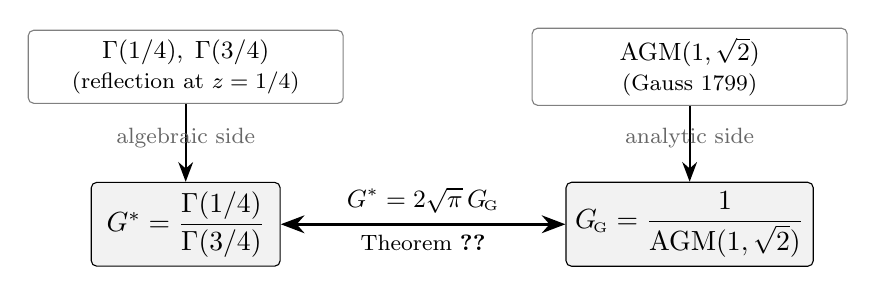
\begin{tikzpicture}[
  source/.style={rectangle, draw=black!50, rounded corners=2pt, minimum width=4cm, minimum height=0.9cm, align=center, font=\small},
  norm/.style={rectangle, draw=black, fill=black!5, rounded corners=2pt, minimum width=2.4cm, minimum height=0.9cm, align=center},
  bridge/.style={very thick, <->, >={Stealth[length=3mm]}},
  feeds/.style={->, >={Stealth[length=2.5mm]}, thick}
]
  % Origin sources (top)
  \node[source] (gamma) at (-3.2, 2) {$\Gamma(1/4),\; \Gamma(3/4)$ \\ \footnotesize (reflection at $z=1/4$)};
  \node[source] (agm)   at ( 3.2, 2) {$\mathrm{AGM}(1, \sqrt 2)$ \\ \footnotesize (Gauss 1799)};
  % Two normalisations (middle)
  \node[norm] (gs) at (-3.2, 0) {$\Gs = \dfrac{\Gamma(1/4)}{\Gamma(3/4)}$};
  \node[norm] (gg) at ( 3.2, 0) {$\GG = \dfrac{1}{\mathrm{AGM}(1,\sqrt 2)}$};
  % Arrows: sources -> normalisations
  \draw[feeds] (gamma) -- (gs);
  \draw[feeds] (agm)   -- (gg);
  % Bridge between normalisations
  \draw[bridge] (gs) -- node[above, font=\small]{$\Gs = 2\sqrt{\pi}\,\GG$} node[below, font=\footnotesize]{Theorem~\ref{thm:bridge}} (gg);
  % Side annotations
  \node[font=\footnotesize, text=black!60] at (-3.2, 1.1) {algebraic side};
  \node[font=\footnotesize, text=black!60] at ( 3.2, 1.1) {analytic side};
\end{tikzpicture}
\caption{Two natural sources, one transcendental, two normalisations. The
lemniscatic CM point generates a single value reachable from either the
\emph{algebraic} Gamma--reflection route (giving $\Gs$) or the
\emph{analytic} AGM route (giving $\GG$); the two normalisations are
related by the bridge $\Gs = 2\sqrt{\pi}\,\GG$. The dichotomy thesis of
this paper is that identities arising on the left side are clean in $\Gs$,
identities on the right side are clean in $\GG$, with a small number of
borderline-period identities clean in both.}\label{fig:bridge}
\end{figure}

\begin{corollary}[Conversion table]\label{cor:conversions}
The following identities convert between $\Gs$, $\GG$, and the lemniscate
constant $\varpi$:
\begin{center}
\begin{tabular}{ll}
\toprule
$\Gs = 2\sqrt{\pi}\,\GG$ & $\GG = \Gs/(2\sqrt\pi)$ \\
$\varpi = \pi\,\GG = \Gs\sqrt\pi/2$ & $\GG = \varpi/\pi$ \\
${\Gs}^{2k} = (4\pi)^k\,{\GG}^{2k}$ & ${\GG}^{2k} = {\Gs}^{2k}/(4\pi)^k$ \\
${\Gs}^{2k+1} = 2^{2k+1}\pi^{k+1/2}\,{\GG}^{2k+1}$ & ${\GG}^{2k+1} = {\Gs}^{2k+1}/(2^{2k+1}\pi^{k+1/2})$ \\
\bottomrule
\end{tabular}
\end{center}
\end{corollary}

Throughout the paper, we adopt the discipline: \emph{express each identity
in the convention in which its coefficients are rational}, with the bridge
identity supplied where conversion is needed. This is the operational
content of Observation~\ref{obs:dichotomy}.

\section{Reflection identities: the algebraic core in $\Gs$}\label{sec:reflect}

\begin{lemma}[Reflection at $z = 1/4$]\label{lem:reflection}
\begin{align}
\Gamma(1/4)^2 &= \pi\sqrt{2}\,\Gs, \label{eq:Gam14sq}\\
\Gamma(3/4)^2 &= \pi\sqrt{2}/\Gs, \label{eq:Gam34sq}\\
\Gamma(1/4)^4 &= 2\pi^2\,\Gss, \label{eq:Gam14fourth}\\
\Gamma(1/4)^8 &= 4\pi^4\,{\Gs}^4. \label{eq:Gam14eighth}
\end{align}
\end{lemma}

\begin{proof}
Euler's reflection \eqref{eq:reflection} at $z = 1/4$:
$\Gamma(1/4)\Gamma(3/4) = \pi/\sin(\pi/4) = \pi\sqrt 2$.
Multiply by $\Gs$ for \eqref{eq:Gam14sq}; divide for \eqref{eq:Gam34sq};
square for \eqref{eq:Gam14fourth} and \eqref{eq:Gam14eighth}.
\end{proof}

\begin{remark}
These four identities exhibit the cleanness of $\Gs$ for the
reflection-channel structure: rational coefficients in $\Gs$
(no $\pi$ inside the coefficient), with $\pi$ appearing only as the
external factor from Euler reflection. The corresponding identities in
$\GG$ have the form $\Gamma(1/4)^2 = (\pi\sqrt 2)(2\sqrt\pi)\GG =
2\sqrt 2\,\pi^{3/2}\GG$, which introduces $\pi^{3/2}$ — fractional powers.
\end{remark}

\begin{corollary}\label{cor:reflection-extras}
The two complementary identities are:
\begin{align}
\Gamma(1/4)\Gamma(3/4) &= \pi\sqrt 2 \quad\text{(product channel, yields $\pi$)}, \\
\Gamma(1/4)/\Gamma(3/4) &= \Gs \quad\text{(ratio channel, yields the new transcendental)}.
\end{align}
The pair $(\Gamma(1/4), \Gamma(3/4))$ is uniquely determined by these two
quantities:
\[
\Gamma(1/4) = \sqrt{\pi\sqrt 2\,\Gs}, \qquad \Gamma(3/4) = \sqrt{\pi\sqrt 2/\Gs}.
\]
\end{corollary}

\section{Three equivalent definitions of $\Gs$}\label{sec:eqdef}

\begin{theorem}[Equivalent definitions]\label{thm:equivalence}
The following are equal:
\begin{enumerate}[label=\textup{(\roman*)}, leftmargin=*]
\item $\Gs = \Gamma(1/4)/\Gamma(3/4)$ (Gamma-ratio form).
\item $\Gs = \sqrt{2\pi}/\AGM(1, 1/\sqrt 2)$ (AGM form).
\item $\Gs = \dfrac{1}{\sqrt{2\pi}}\int_0^1 \dfrac{dt}{[t(1-t)]^{3/4}}$
(Beta-integral form).
\end{enumerate}
\end{theorem}

\begin{proof}
(i)\,$=$\,(iii): The Beta integral gives $B(1/4, 1/4) = \Gamma(1/4)^2/\sqrt\pi$.
By \eqref{eq:Gam14sq}, $\Gamma(1/4)^2 = \pi\sqrt 2\,\Gs$, so
$B(1/4, 1/4) = \sqrt{2\pi}\,\Gs$, equivalent to (iii).

(i)\,$=$\,(ii): By homogeneity $\AGM(\lambda a, \lambda b) = \lambda\AGM(a,b)$,
$\AGM(1, 1/\sqrt 2) = \AGM(\sqrt 2, 1)/\sqrt 2 = \AGM(1,\sqrt 2)/\sqrt 2$.
By Theorem~\ref{thm:bridge}, $\AGM(1,\sqrt 2) = 1/\GG = 2\sqrt\pi/\Gs$, so
$\AGM(1, 1/\sqrt 2) = \sqrt{2\pi}/\Gs$, which gives (ii).
\end{proof}

\begin{remark}
Definition (i) is the algebraic-reflection form. Definition (ii) gives
the bridge to $\GG$: rewriting (ii),
$\Gs = \sqrt{2\pi} \cdot \sqrt 2 \cdot \GG = 2\sqrt\pi\,\GG$, which
recovers \eqref{eq:bridge}. Definition (iii) is the period-integral form
relevant for Kontsevich--Zagier (\S\ref{sec:KZ}). The AGM definition (ii)
also admits a Borwein-like self-replicating algorithmic generalisation
that computes $\Gs$ (via $\Gamma(1/4)$) to arbitrary precision; see
Guillera \cite{guillera-selfreplication} for the self-replication
framework that extends the Borwein algorithms for $\pi$
\cite{borweinAGM} to $\Gamma$-values at rational arguments including
$\Gamma(1/4)$ and $\Gamma(1/3)$.
\end{remark}

\section{The lemniscatic elliptic curve}\label{sec:lemniscatic}

\begin{definition}
The lemniscatic elliptic curve over $\Q$ is $E: y^2 = x^3 - x$.
\end{definition}

\begin{lemma}\label{lem:E-properties}
$E$ has complex multiplication by $\Z[i]$, $j$-invariant $1728$, discriminant
$64$, and $|\Aut_\C(E)| = 4$, with the automorphism group generated by
$(x,y) \mapsto (-x, iy)$.
\end{lemma}

\begin{theorem}[Real period]\label{thm:period}
The real period of $E$ admits the four equivalent expressions:
\begin{align}
\omega_E &= 2\int_{-1}^{0} \frac{dx}{\sqrt{x(x-1)(x+1)}} \\
&= \frac{\Gamma(1/4)^2}{\sqrt{2\pi}} \quad \text{(Gamma form)} \\
&= \Gs\sqrt\pi \quad \text{(reflection form, in $\Gs$)} \\
&= 2\pi\,\GG \quad \text{(AGM form, in $\GG$)}.
\end{align}
All four forms have rational or simple algebraic coefficients. The
$\Gs$-form and $\GG$-form are both clean: $\omega_E$ is a borderline
identity natural in either normalisation
(see Observation~\ref{obs:period-borderline}).
\end{theorem}

\begin{proof}
The integral evaluation $\omega_E = \Gamma(1/4)^2/\sqrt{2\pi}$ is classical;
see \cite[\S 2.5]{borweinAGM}. The $\Gs$-form follows from
$\Gamma(1/4)^2 = \pi\sqrt 2\,\Gs$ (Lemma~\ref{lem:reflection}).
The $\GG$-form follows from the bridge identity $\Gs = 2\sqrt\pi\,\GG$:
$\omega_E = \Gs\sqrt\pi = (2\sqrt\pi\,\GG)\,\sqrt\pi = 2\pi\,\GG$.
\end{proof}

\begin{observation}\label{obs:period-borderline}
Theorem~\ref{thm:period} reveals that $\omega_E = 2\pi\GG$ has \emph{clean
integer coefficient} in $\GG$ (the period is literally $2\pi$ times Gauss's
constant) but \emph{also} has clean form $\Gs\sqrt\pi$. This is one of the
borderline identities where both conventions are reasonable. The
lemniscatic period sits exactly at the algebraic-analytic boundary:
it is the period of an algebraic curve (algebraic origin, hence $\Gs$
representation $\omega_E = \Gs\sqrt\pi$ is natural) but also $2\pi$ times
the reciprocal of $\AGM(1, \sqrt 2)$ (analytic origin, hence
$\omega_E = 2\pi\GG$). Both forms are integer-coefficient.
\end{observation}

\section{The master quadratic: the algebraic centerpiece}\label{sec:masterq}

Consider the polynomial
\begin{equation}
\boxed{\;P_{\!\Gs}(x) \;:=\; x^2 - 16\,\Gss\,x + 16\,\Gsss\;} \label{eq:MQ}
\end{equation}
with integer coefficient $16$.

\begin{theorem}[Master quadratic structure]\label{thm:MQ}
The polynomial $P_{\!\Gs}(x)$ has positive discriminant
$256\,{\Gs}^4 - 64\,{\Gs}^3 = 64\,{\Gs}^3(4\Gs - 1) > 0$ and roots
\[
x_\pm \;=\; 8\,\Gss \,\pm\, 4\,{\Gs}^{3/2}\sqrt{4\Gs - 1}.
\]
Numerically:
\begin{align}
x_+ &= 137.03617145815548388\ldots, \\
x_- &= 3.02396391633902100\ldots
\end{align}
Vieta's identities give
\begin{equation}
\frac{1}{x_+} + \frac{1}{x_-} = \frac{1}{\Gs}, \qquad
x_+ \cdot x_- = 16\,\Gsss.
\label{eq:vieta}
\end{equation}
\end{theorem}

\begin{proof}
Direct computation via the quadratic formula and Vieta's identities.
\end{proof}

\begin{observation}[Integer-coefficient signature]\label{obs:MQ-integer}
The polynomial $P_{\!\Gs}$ has integer coefficients in $\Gs$. The
coefficient $16 = |\Aut_\C(E)|^2$ is the squared automorphism count of the
lemniscatic curve. In $\GG$-coordinates, the same polynomial becomes
\[
x^2 - 64\pi\,{\GG}^2\,x + 128\pi^{3/2}\,{\GG}^3,
\]
with explicit $\pi$ and $\pi^{3/2}$ in the coefficients. The integer $16$
disappears; the algebraic identification with $|\Aut(E)|^2$ is obscured.
This is the cleanest illustration of Observation~\ref{obs:dichotomy}:
the master quadratic is intrinsically a $\Gs$ object.
\end{observation}

\begin{remark}[Numerical content of the roots]\label{rem:MQ-numerical}
The roots take the numerical values $x_+ \approx 137.036$ and
$x_- \approx 3.024$. Their identification with physical observables
and the resulting math--physics bridge lie outside the mathematical
scope of the present paper and are treated in a separate note in
preparation. The transcendence and algebraic-independence
implications of the roots are addressed in \S\ref{sec:transcendence}.
\end{remark}

\section{Beta integrals at quarter arguments}\label{sec:beta}

\begin{lemma}\label{lem:beta-quarter}
The Beta function at $(1/4, 1/4)$ admits the closed forms:
\begin{align}
B(1/4, 1/4) &= \int_0^1 [t(1-t)]^{-3/4}\,dt \\
&= \frac{\Gamma(1/4)^2}{\Gamma(1/2)} \;=\; \frac{\Gamma(1/4)^2}{\sqrt\pi} \\
&= \sqrt{2\pi}\,\Gs \quad \text{(in $\Gs$, clean)}\\
&= 2\sqrt 2\,\pi\,\GG \quad \text{(in $\GG$, integer-coefficient).}
\end{align}
\end{lemma}

\begin{proof}
The Beta-integral evaluation is classical: $B(p,q) = \Gamma(p)\Gamma(q)/\Gamma(p+q)$.
At $p = q = 1/4$, $\Gamma(p+q) = \Gamma(1/2) = \sqrt\pi$. The $\Gs$-form
follows from \eqref{eq:Gam14sq}. The $\GG$-form follows from \eqref{eq:bridge}:
$\sqrt{2\pi}\,\Gs = \sqrt{2\pi}\cdot 2\sqrt\pi\,\GG = 2\sqrt{2\pi^2}\,\GG = 2\sqrt 2\,\pi\,\GG$.
\end{proof}

\begin{remark}
This is another borderline identity where both forms are clean: $\Gs$ gives
$\sqrt{2\pi}$ as coefficient (irrational but classical), $\GG$ gives $4\pi$
(integer multiple of $\pi$). Both are rational-coefficient identities in
their respective constants. The Beta integral, like the lemniscatic period
\eqref{thm:period}, sits at the boundary.
\end{remark}

\section{The family $R_n$ and the distinguishedness of $R_4 = \Gs$}\label{sec:family}

\begin{definition}
For integer $n \geq 2$, $R_n := \Gamma(1/n)/\Gamma((n-1)/n)$.
\end{definition}

\begin{proposition}\label{prop:Rn-family}
The family $\{R_n\}_{n \geq 2}$ satisfies:
\begin{enumerate}[label=\textup{(\roman*)}, leftmargin=*, itemsep=2pt]
\item $R_n > 0$ for all $n \geq 2$;
\item $R_n = \Gamma(1/n)^2 \sin(\pi/n)/\pi$ (by Euler reflection);
\item $R_2 = 1$ (trivially) and $R_n = n - 2\gamma + O(1/n)$ as $n \to \infty$,
where $\gamma$ is the Euler--Mascheroni constant.
\end{enumerate}
The first six values:
\begin{center}
\begin{tabular}{rl@{\qquad}l}
\toprule
$n$ & $R_n$ & associated CM-curve interpretation \\
\midrule
$2$ & $1.0000000000$  & trivial \\
$3$ & $1.9783642596\ldots$ & equianharmonic $E: y^2 = x^3 - 1$, $\mathrm{End}(E) = \Z[\rho]$, $|\Aut| = 6$ \\
$4$ & $2.9586751192\ldots\;\;(\Gs)$ & lemniscatic $E: y^2 = x^3 - x$, $\mathrm{End}(E) = \Z[i]$, $|\Aut| = 4$ \\
$5$ & $3.9432456137\ldots$ & no CM curve with this argument structure \\
$6$ & $4.9312366764\ldots$ & equianharmonic via twist $y^2 = x^3 + 1$ \\
$8$ & $6.9140781897\ldots$ & no CM curve \\
\bottomrule
\end{tabular}
\end{center}
\end{proposition}

\begin{theorem}[Algebraic distinguishedness of $R_4$]\label{thm:R4-distinguished}
Among the $R_n$ family with $n \in \{2, 3, 4, 5, 6, 8, 12\}$, the value
$R_4 = \Gs$ is the unique value such that $R_n$ is the gamma-ratio of a
class-number-one CM elliptic curve over $\Q$ with $|\Aut_{\C}(E)|^{2} = 16$.
The equianharmonic curve $E_\rho$ at $R_3$ (and its twist at $R_6$) has
$|\Aut_{\C}(E_\rho)|^{2} = 36$; no other $R_n$ in the listed range
corresponds to a CM elliptic curve with extra automorphisms.
\end{theorem}

\begin{proof}
Direct enumeration. The class-number-one imaginary-quadratic fields with
unit group strictly larger than $\{\pm 1\}$ are exactly $\Q(i)$ (units of
order $4$) and $\Q(\rho)$ (units of order $6$). These yield the
lemniscatic curve $y^2 = x^3 - x$ over $\Q$, with $R_4 = \Gamma(1/4)/\Gamma(3/4)$
and $|\Aut|^{2} = 16$, and the equianharmonic curve $y^2 = x^3 - 1$ (with
twist $y^2 = x^3 + 1$), with $R_3 = \Gamma(1/3)/\Gamma(2/3)$ (resp.\ $R_6$)
and $|\Aut|^{2} = 36$. For $n \in \{2, 5, 8, 12\}$, no CM elliptic curve
over $\Q$ has $R_n$ as its gamma-ratio.
\end{proof}

\begin{observation}[Numerical content of the roots at $R_4$ and $R_3$]\label{obs:Rn-numerical}
Numerical evaluation of $x_\pm(R_n) = (16 R_n^2 \pm \sqrt{(16 R_n^2)^2 - 64 R_n^3})/2$
for the CM-relevant values $R_3, R_4, R_6$ yields:
\[
\begin{array}{lccc}
\toprule
n & R_n & x_+(R_n) & x_-(R_n) \\
\midrule
3 & 1.97836 & 138.894\,\ldots & 2.007\,\ldots \\
4 & 2.95868\;(\Gs) & 137.036\,\ldots & 3.024\,\ldots \\
6 & 4.93124 & 384.078\,\ldots & 4.995\,\ldots \\
\bottomrule
\end{array}
\]
(In rows $3, 6$ the polynomial coefficient is $16 R_n^2 / 16 R_n^3$ as in the
lemniscatic case; the corresponding equianharmonic master quadratic
$y^2 - 36 R_n^2 y + 36 R_n^3$ would have $|\Aut|^{2} = 36$ as its integer
prefactor.) Their interpretation as physical observables is addressed in
a separate note in preparation.
\end{observation}

\begin{proposition}[Family-wide master-quadratic root asymptotic, with full expansion]\label{prop:Rn-asymptotic}
For the master-quadratic family
$x^2 - 16 R^2 x + 16 R^3 = 0$ with $R > 1/4$, the smaller root admits the
absolutely convergent expansion
\[
x_-(R) \;=\; \sum_{n=1}^\infty d_n\,R^{2-n}, \qquad
d_n \;=\; \frac{\binom{2n}{n}}{(2n-1)\,2^{4n-3}},
\]
giving explicit leading terms
\[
x_-(R) \;=\; R \;+\; \frac{1}{16} \;+\; \frac{1}{128\,R} \;+\; \frac{5}{4096\,R^2}
            \;+\; \frac{7}{32768\,R^3} \;+\; O(R^{-4}).
\]
The larger root satisfies $x_+(R) = 16 R^2 - x_-(R)$ by Vieta, hence
$x_+(R) = 16 R^2 - R - 1/16 - 1/(128R) - O(R^{-2})$.
\end{proposition}

\begin{proof}
Write the quadratic formula in the form
$x_-(R) = 8 R^2\,\bigl(1 - \sqrt{1 - y}\bigr)$ with $y = 1/(4R) \in (0, 1)$.
The Newton binomial expansion gives
$1 - \sqrt{1 - y} = \sum_{n \geq 1} c_n'\, y^n$
with $c_n' = \binom{2n}{n}/\bigl((2n-1)\,4^n\bigr)$ for $n \geq 1$, so
\[
x_-(R) \;=\; 8 R^2 \sum_{n \geq 1} \frac{c_n'}{(4R)^n}
       \;=\; \sum_{n \geq 1} \frac{8\,c_n'}{4^n}\,R^{2-n}
       \;=\; \sum_{n \geq 1} d_n\, R^{2-n},
\]
where $d_n := 8\,c_n'/4^n = \binom{2n}{n}/\bigl((2n-1)\,2^{4n-3}\bigr)$.
Direct evaluation: $d_1 = 1$, $d_2 = 1/16$, $d_3 = 1/128$, $d_4 = 5/4096$,
$d_5 = 7/32768$, recovering the leading $R$ and the four subsequent
correction terms. Convergence for $4R > 1$ is by ratio test:
$|d_{n+1}\,R^{-1}/d_n| \to 1/(4R) < 1$.
\end{proof}

\begin{remark}[Numerical verification across $R_n$]\label{rem:asym-numerics}
The difference $x_-(R_n) - R_n$ approaches $1/16 = 0.0625$ from above:
\begin{center}
\begin{tabular}{rlll}
\toprule
$n$ & $R_n$ & $x_-(R_n)$ & $x_-(R_n) - R_n$ \\
\midrule
$3$ & $1.97836$ & $2.04516$ & $0.06680$ \\
$4$ & $2.95868\;\;(\Gs)$ & $3.02396$ & $0.06528$ \\
$5$ & $3.94325$ & $4.00781$ & $0.06456$ \\
$6$ & $4.93124$ & $4.99537$ & $0.06413$ \\
$8$ & $6.91408$ & $6.97773$ & $0.06366$ \\
$12$ & $10.89429$ & $10.95752$ & $0.06323$ \\
$\infty$ & ($n - 2\gamma$) & ($\to R_n + 1/16$) & $1/16 = 0.06250$ \\
\bottomrule
\end{tabular}
\end{center}
The constant excess $x_-(R_n) - R_n \to 1/16$ as $n \to \infty$ is a
structural feature of the family $x^2 - 16 R^2 x + 16 R^3 = 0$ and is
independent of any physical interpretation of the roots
(Figure~\ref{fig:Rn-asymptote}).

\begin{figure}[ht]
\centering
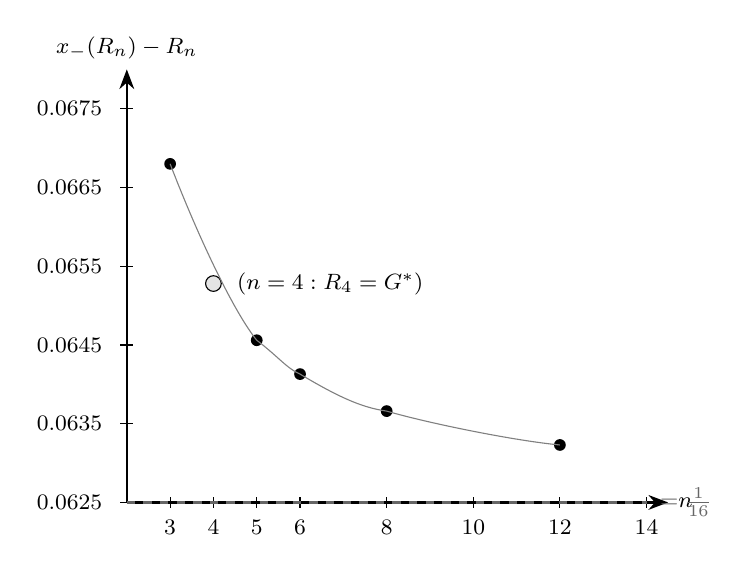
\begin{tikzpicture}[
  xscale=0.55,
  yscale=1.0,
  axis/.style={->, >={Stealth[length=2.5mm]}, thick},
  point/.style={circle, fill=black, inner sep=1.5pt},
  highlight/.style={circle, draw=black, fill=black!10, inner sep=2pt}
]
  % Axes: x in [2, 14], y in [0, 5] (scaled units of 0.001 each, representing 0.0625 + y/1000)
  \draw[axis] (2, 0) -- (14.5, 0) node[right, font=\footnotesize] {$n$};
  \draw[axis] (2, 0) -- (2, 5.5) node[above, font=\footnotesize] {$x_-(R_n) - R_n$};
  % y-axis tick labels
  \foreach \y/\label in {0/{$0.0625$}, 1/{$0.0635$}, 2/{$0.0645$}, 3/{$0.0655$}, 4/{$0.0665$}, 5/{$0.0675$}} {
    \draw (1.85, \y) -- (2.15, \y);
    \node[left, font=\footnotesize, xshift=-3pt] at (1.85, \y) {\label};
  }
  % x-axis tick labels
  \foreach \x in {3,4,5,6,8,10,12,14} {
    \draw (\x, -0.07) -- (\x, 0.07);
    \node[below, font=\footnotesize] at (\x, -0.1) {\x};
  }
  % Asymptote line at y = 0 (actual value 1/16 = 0.0625)
  \draw[dashed, black!60, thick] (2, 0) -- (14, 0);
  \node[font=\footnotesize, text=black!60, right] at (14, 0) {$\,= \tfrac{1}{16}$};
  % Data points (n, scaled_excess)
  \node[point] at (3,  4.30) {};
  \node[point] at (4,  2.78) {};
  \node[point] at (5,  2.06) {};
  \node[point] at (6,  1.63) {};
  \node[point] at (8,  1.16) {};
  \node[point] at (12, 0.73) {};
  % Highlight n=4 (= G*)
  \node[highlight, label={[font=\footnotesize, label distance=2pt]right:$(n=4: R_4 = \Gs)$}] at (4, 2.78) {};
  % Smooth qualitative curve connecting the points (monotone decreasing toward asymptote)
  \draw[black!50, thin] (3, 4.30) .. controls (3.7, 3.3) and (4.5, 2.4) .. (5, 2.06)
                                  .. controls (5.5, 1.85) and (5.7, 1.7) .. (6, 1.63)
                                  .. controls (7, 1.3) and (7.5, 1.2) .. (8, 1.16)
                                  .. controls (9, 1.0) and (11, 0.78) .. (12, 0.73);
\end{tikzpicture}
\caption{Numerical convergence $x_-(R_n) - R_n \to 1/16$ from above for
$n \in \{3, 4, 5, 6, 8, 12\}$. The asymptote at $1/16 \approx 0.0625$
(dashed) is the structural feature of the family $x^2 - 16 R^2 x + 16 R^3 = 0$
identified in Proposition~\ref{prop:Rn-asymptotic}: the leading correction
$d_2 = 1/16$ is constant in $R$, with subsequent corrections of order
$R^{-1}, R^{-2}, \ldots$ The lemniscatic point $R_4 = \Gs$ is highlighted;
its value $x_-(\Gs) - \Gs \approx 0.06528$ is the $n = 4$ instance of the
family-wide asymptotic.}\label{fig:Rn-asymptote}
\end{figure}
\end{remark}

\section{The Watson lattice identity, in $\GG$}\label{sec:watson}

We now cross the algebraic--analytic boundary. The body-centred-cubic
lattice Green's function at the origin admits the cleanest expression
in $\GG$:

\begin{theorem}[Watson 1939, restated in $\GG$]\label{thm:watson}
The body-centred-cubic lattice Green's function at the origin satisfies
\begin{equation}
W^{(3)}_{\mathrm{BCC}} \;:=\; \frac{1}{\pi^3}\int_0^\pi\!\!\int_0^\pi\!\!\int_0^\pi \frac{dk_1\,dk_2\,dk_3}{1 - \cos k_1 \cos k_2 \cos k_3} \;=\; 2\,{\GG}^2 \;=\; \frac{2}{\AGM(1, \sqrt 2)^2}.
\label{eq:watson}
\end{equation}
\end{theorem}

\begin{observation}
The form $W^{(3)}_{\mathrm{BCC}} = 2/\AGM(1, \sqrt 2)^{2}$ states
directly that the BCC random walk's expected returns-to-origin count
is computable by Gauss's AGM applied to $(1, \sqrt 2)$, with no
occurrence of $\pi$ or $\Gamma$. The standard form is
$\Gamma(1/4)^{4}/(4\pi^{3})$ \cite{watson1939, vanPeype}; the
intermediate form $W^{(3)}_{\mathrm{BCC}} = (4/\pi^{2})\,K(1/\sqrt 2)^{2}$
is also classical (cf.\ \cite{borweinAGM} for the AGM substitution
$K(1/\sqrt 2) = \pi\GG/\sqrt 2$). The author has not located the
fully-reduced $\AGM$-form \eqref{eq:watson} in the surveyed
literature (Watson 1939, van Peype 1938, Joyce 1971, Borwein--Borwein
1987, Guttmann 2010), but does not claim it is novel; the substitution
is one step from the references cited.
\end{observation}

\begin{proof}
The classical reduction \cite{watson1939} gives
$W^{(3)}_{\mathrm{BCC}} = (4/\pi^2)\,K(1/\sqrt 2)^2$.
The AGM evaluation $K(1/\sqrt 2) = \pi\,\GG/\sqrt 2$ (Theorem~\ref{thm:elliptic})
then yields
\[
W^{(3)}_{\mathrm{BCC}} \;=\; \frac{4}{\pi^2} \cdot \frac{\pi^2\,{\GG}^2}{2}
                       \;=\; 2\,{\GG}^2. \qedhere
\]
\end{proof}

\begin{theorem}[Generalised Watson identity; Guttmann 2010]\label{thm:gen-watson}
For all integer $D \geq 3$, the $D$-dimensional body-centred-cubic Watson
integral equals the hypergeometric series
\begin{equation}
W^{(D)}_{\mathrm{BCC}} \;=\; {}_DF_{D-1}\!\left(\tfrac12, \tfrac12, \ldots, \tfrac12; 1, 1, \ldots, 1; 1\right) \;=\; \sum_{n=0}^\infty \binom{2n}{n}^{\!D} \frac{1}{16^{n}}\!\cdot\!\frac{1}{2^{n(D-2)}}.
\label{eq:gen-watson}
\end{equation}
\end{theorem}

\begin{proof}
Expand $1/(1 - \prod \cos k_i)$ as geometric series, integrate term-by-term
using $\int_0^\pi (\cos k)^{2m}\,dk = \pi\,(1/2)_m/m!$, and recognise the
resulting series as the hypergeometric. Convergence at $z = 1$ requires
$D \geq 3$. The derivation in this form is due to Guttmann
\cite[\S2.1]{guttmann2010}, who also gives the equivalent multinomial expression.
\end{proof}

\begin{corollary}[Numerical values, $D = 3, 4, 5$]\label{cor:WD-numerics}
To 20 decimal digits:
\begin{align*}
W^{(3)}_{\mathrm{BCC}} &= 2\,{\GG}^2 = 1.39320392968567685918\ldots, \\
W^{(4)}_{\mathrm{BCC}} &= {}_4F_3(\tfrac12{}^4; 1^3; 1) = 1.11863638716418706835\ldots, \\
W^{(5)}_{\mathrm{BCC}} &= {}_5F_4(\tfrac12{}^5; 1^4; 1) = 1.04682554983350000525\ldots.
\end{align*}
\end{corollary}

\begin{remark}
The $D = 3$ case admits the closed form $2{\GG}^2$; the cases $D \geq 4$ do not
admit any known closed form in elementary functions or values of $\Gamma$.
PSLQ search to 30+ digit precision finds no integer relation between
$W^{(4)}_{\mathrm{BCC}}$ and any rational power product of
$\{\Gs, \GG, \pi, \Gamma(1/4), R_3, R_5, R_6\}$ with coefficient bound
$10^{12}$.
\end{remark}

\section{Theta functions at $\tau = i$, in $\GG$}\label{sec:theta}

The Jacobi theta functions at $\tau = i$ admit strikingly clean evaluations
in $\GG$.

\begin{theorem}[Theta values at $\tau = i$]\label{thm:theta-values}
With the Jacobi conventions, at the lemniscatic CM point $\tau = i$:
\begin{align}
\theta_2(0\,|\,i)^2 &= \GG, \label{eq:theta2sq}\\
\theta_3(0\,|\,i)^2 &= \sqrt{2}\,\GG, \label{eq:theta3sq}\\
\theta_4(0\,|\,i)^2 &= \GG. \label{eq:theta4sq}
\end{align}
Equivalently $\theta_2(0\,|\,i) = \theta_4(0\,|\,i) = \sqrt{\GG}$ and
$\theta_3(0\,|\,i) = 2^{1/4}\sqrt{\GG}$. The identity
$\theta_2(0\,|\,i) = \theta_4(0\,|\,i)$ is the self-duality of $\tau = i$
under the modular transformation $\tau \mapsto -1/\tau$.
\end{theorem}

\begin{proof}
The classical evaluations at $\tau = i$ are
$\theta_3(0\,|\,i) = \pi^{1/4}/\Gamma(3/4)$ and
$\theta_2(0\,|\,i) = \theta_4(0\,|\,i) = \pi^{1/4}/(2^{1/4}\,\Gamma(3/4))$
(see e.g.\ \cite[\S{}21.5]{whittaker-watson} or \cite[Eq.~2.7.6]{borweinAGM}).
Squaring $\theta_3$ and applying \eqref{eq:Gam34sq}:
\[
\theta_3(0\,|\,i)^2 = \frac{\sqrt\pi}{\Gamma(3/4)^2}
                    = \frac{\sqrt\pi}{\pi\sqrt 2/\Gs}
                    = \frac{\Gs}{\sqrt{2\pi}}.
\]
Using $\Gs = 2\sqrt\pi\,\GG$ from Theorem~\ref{thm:bridge}:
$\theta_3(0\,|\,i)^2 = 2\sqrt\pi\,\GG/\sqrt{2\pi} = \sqrt 2\,\GG$.
Similarly, $\theta_2(0\,|\,i)^2 = \theta_4(0\,|\,i)^2 = \sqrt{\pi}/(\sqrt 2\,\Gamma(3/4)^2)
= \GG$ (the factor of $\sqrt 2$ relative to $\theta_3^2$).
\end{proof}

\begin{corollary}\label{cor:theta-higher}
For all integer $k \geq 1$,
$\theta_2(0\,|\,i)^{2k} = \theta_4(0\,|\,i)^{2k} = \GG^k$ and
$\theta_3(0\,|\,i)^{2k} = 2^{k/2}\,\GG^k$.
\end{corollary}

\begin{remark}[Jacobi's identity at $\tau = i$]
Jacobi's identity $\theta_3^4 = \theta_2^4 + \theta_4^4$ at $\tau = i$ becomes
$2\GG^2 = \GG^2 + \GG^2$, which is trivially satisfied by the self-duality
$\theta_2(0\,|\,i) = \theta_4(0\,|\,i)$. The modular lambda function
$\lambda(\tau) = \theta_2^4/\theta_3^4$ evaluates to
$\lambda(i) = \GG^2/(2\GG^2) = 1/2$, recovering the classical value at the
self-complementary modulus.
\end{remark}

\section{The Dedekind eta at $\tau = i$, in $\GG$}\label{sec:eta}

\begin{theorem}[Chowla--Selberg at $\tau = i$, restated in $\GG$]\label{thm:eta-i}
\[
\eta(i) \;=\; \frac{{\GG}^{1/2}}{2^{1/4}} \;=\; \frac{1}{2^{1/4}\,\AGM(1,\sqrt 2)^{1/2}}.
\]
\end{theorem}

\begin{proof}
The Chowla--Selberg evaluation at $K = \Q(i)$ gives $\eta(i) =
\Gamma(1/4)/(2\pi^{3/4})$ \cite{chowlaselberg,cohenII}. Substituting
$\Gamma(1/4) = \sqrt{\pi\sqrt 2\,\Gs}$ (from Cor.~\ref{cor:reflection-extras}):
\[
\eta(i) \;=\; \frac{\sqrt{\pi\sqrt 2\,\Gs}}{2\pi^{3/4}} \;=\; \frac{\pi^{1/2} 2^{1/4} {\Gs}^{1/2}}{2\pi^{3/4}} \;=\; \frac{2^{1/4}\,{\Gs}^{1/2}}{2\,\pi^{1/4}} \;=\; \frac{{\Gs}^{1/2}}{2^{3/4}\,\pi^{1/4}}.
\]
Using $\Gs = 2\sqrt\pi\,\GG$, we have ${\Gs}^{1/2} = 2^{1/2}\pi^{1/4}{\GG}^{1/2}$, so
\[
\eta(i) \;=\; \frac{2^{1/2}\pi^{1/4}\,{\GG}^{1/2}}{2^{3/4}\,\pi^{1/4}} \;=\; \frac{{\GG}^{1/2}}{2^{1/4}}. \qedhere
\]
\end{proof}

\begin{corollary}\label{cor:eta-powers}
The following powers of $\eta(i)$ have clean expressions in $\GG$:
\begin{align*}
\eta(i) &= 2^{-1/4}\,{\GG}^{1/2}, \\
\eta(i)^2 &= 2^{-1/2}\,\GG, \\
\eta(i)^4 &= 2^{-1}\,{\GG}^2 = {\GG}^2/2, \\
\eta(i)^8 &= {\GG}^4/4, \\
\eta(i)^{12} &= {\GG}^6/8, \\
\eta(i)^{24} &= {\GG}^{12}/64.
\end{align*}
\end{corollary}

\begin{corollary}[Watson--eta bridge]\label{cor:watson-eta}
\[
W^{(3)}_{\mathrm{BCC}} \;=\; 4\,\eta(i)^4 \;=\; 2\,{\GG}^2.
\]
\end{corollary}

\subsection{The $\eta$ half-tower at related CM points}

\begin{theorem}[$\eta$ at $i/2$ and $2i$]\label{thm:eta-half-tower}
\begin{align}
\eta(i/2)^2 &= \GG / 2^{1/4}, \\
\eta(i)^2 &= \GG / 2^{1/2}, \\
\eta(2i)^2 &= \GG / 2^{5/4}.
\end{align}
The first and third are linked by the modular $S$-transformation:
$\eta(i/2) = \sqrt 2\,\eta(2i)$. The tower of clean $\GG$-form values
\emph{stops} at $\tau = 2i$: $\eta(4i)^2/\GG = 0.14685\ldots$ is not
$2^{-n}$ for any rational $n$, because $\tau = 4i$ is a CM point of the
conductor-$2$ order in $\Z[i]$, not the maximal order. The fundamental
period of that order is a different transcendental.
\end{theorem}

\begin{proof}
Apply $\eta(2i) = \Gamma(1/4)/(2^{11/8}\pi^{3/4})$ and the bridge identity
$\Gamma(1/4)^2 = 2\pi\sqrt{2\pi}\,\GG$ to obtain
$\eta(2i)^2 = \GG/2^{5/4}$. The modular transformation
$\eta(-1/\tau) = \sqrt{-i\tau}\,\eta(\tau)$ at $\tau = 2i$ gives
$\eta(i/2) = \sqrt 2\,\eta(2i)$.
\end{proof}

\begin{corollary}[A clean low-weight $\eta$-product identity]\label{cor:eta-low-weight}
\[
2\,\eta(2i)\,\eta(i/2)^{3} \;=\; \GG^{2}.
\]
\end{corollary}

\begin{proof}
Square both sides and use Theorem~\ref{thm:eta-half-tower}:
$\bigl(2\,\eta(2i)\,\eta(i/2)^{3}\bigr)^{2}
   = 4\,\eta(2i)^{2}\,\eta(i/2)^{6}
   = 4 \cdot \GG/2^{5/4} \cdot \GG^{3}/2^{3/4}
   = 4\,\GG^{4}/2^{2} = \GG^{4}$.
Both sides positive, so the un-squared identity holds.
\end{proof}

\subsection{The first lemniscate constant as a Hecke $L$-value}\label{sec:Lvalue}

\begin{theorem}[$L(E_{\mathrm{lemn}}, 1) = \varpi/4$]\label{thm:Lvalue}
For the lemniscatic elliptic curve $E: y^2 = x^3 - x$ over $\Q$:
\[
L(E, 1) \;=\; \frac{\varpi}{4} \;=\; \frac{\pi\,\GG}{4}.
\]
The closed-form expression of $L(E, 1)$ in terms of $\varpi$ for CM elliptic
curves is classical; the algebraic-part formulation underlying the BSD-style
computation below is treated, for related CM Hecke $L$-series, by
Rodriguez Villegas and Zagier \cite{villegas-zagier}.
\end{theorem}

\begin{proof}
$E$ has analytic rank $0$ with $|\Sha(E/\Q)| = 1$, Tamagawa number
$c_{2} = 2$ at the bad prime $p = 2$ (Kodaira type III on the minimal
model \cite[curve 32.a3]{lmfdb}), torsion subgroup
$E(\Q)_{\mathrm{tors}} = (\Z/2\Z)^{2}$ of order $4$, and two real
connected components at $x \in [-1, 0]$ and $x \in [1, \infty)$. The
real period over the full real locus is
\[
\Omega \;=\; \int_{E(\R)} |dx/y|
       \;=\; 2 \int_{1}^{\infty} \frac{dx}{\sqrt{x^{3} - x}}
       \;=\; 2\varpi \;=\; 2\pi\GG,
\]
where the factor of $2$ counts the two real components. The
Birch--Swinnerton-Dyer formula for rank $0$, proved unconditionally
for CM elliptic curves over $\Q$ by Rubin \cite{rubin1991} (using
Kolyvagin's Euler-system machinery to establish the full quantitative
Birch--Swinnerton-Dyer ratio), gives
\[
L(E, 1) \;=\; \frac{\Omega \cdot \prod_{p} c_{p} \cdot |\Sha|}
              {|E(\Q)_{\mathrm{tors}}|^{2}}
       \;=\; \frac{2\varpi \cdot 2 \cdot 1}{16}
       \;=\; \frac{\varpi}{4}.
\]
\end{proof}

\begin{remark}
The numerical value $L(E_{\mathrm{lemn}}, 1) = \varpi/4 \approx 0.6555144\ldots$
agrees with the LMFDB tabulated value for curve $32.a3$ to all listed
digits.
\end{remark}

\subsection{Complete elliptic integrals at $k = 1/\sqrt 2$}\label{sec:elliptic}

\begin{theorem}[Elliptic integrals at the self-complementary modulus]\label{thm:elliptic}
At $k = 1/\sqrt 2$:
\begin{align}
K(1/\sqrt 2) &= \frac{\pi\,\GG}{\sqrt 2}, \\
E(1/\sqrt 2) &= \frac{\sqrt 2}{4}\!\left(\frac{1}{\GG} + \pi\,\GG\right), \\
K(1/\sqrt 2)\,E(1/\sqrt 2) &= \frac{\pi + \varpi^2}{4}.
\end{align}
\end{theorem}

\begin{proof}
The Legendre relation at $k = k' = 1/\sqrt 2$ becomes $2KE - K^2 = \pi/2$,
so $E = (\pi/2 + K^2)/(2K)$. Substituting the closed form for $K$ gives
$E$. The product $KE$ follows by multiplication and $\varpi = \pi\GG$.
\end{proof}

\begin{corollary}[Inverse identity: $\GG$ from elliptic integrals]\label{cor:GG-inverse}
\[
\GG^2 \;=\; \frac{4\,K(1/\sqrt 2)\,E(1/\sqrt 2) - \pi}{\pi^2}.
\]
This expresses $\GG$ in terms of two independent elliptic-integral evaluations
at the lemniscatic modulus, without reference to $\Gamma$ or the AGM.
\end{corollary}

\begin{proof}
From Theorem~\ref{thm:elliptic}, $K(1/\sqrt 2)\,E(1/\sqrt 2) = (\pi + \varpi^2)/4$
with $\varpi = \pi\,\GG$, so $\varpi^2 = \pi^2\,\GG^2$ and
$4\,K(1/\sqrt 2)\,E(1/\sqrt 2) = \pi + \pi^2\,\GG^2$. Solving for $\GG^2$
gives the stated identity.
\end{proof}

\section{Modular forms at $\tau = i$, in $\GG$}\label{sec:modforms}

The cleanest expression of modular invariants at $\tau = i$ is in $\GG$.
The catalogue below collects standard CM-modular-form values at $\tau = i$;
several of the closed forms (notably $E_4(i) = 3\GG^4$ and $\Delta(i) = \GG^{12}/64$)
appear in Yui--Zagier's tabulation of singular Weber-modular values
\cite{yui-zagier}.

\begin{theorem}[Catalogue of level-one modular invariants at $\tau = i$]\label{thm:catalogue}
For the standard generators of $M_*(\mathrm{SL}_2(\Z))$:
\begin{align}
E_4(i) &= 3\,{\GG}^4, \\
E_6(i) &= 0, \\
E_8(i) &= E_4(i)^2 = 9\,{\GG}^8, \\
E_{10}(i) &= 0, \\
E_{12}(i) &= \frac{441}{691}\,E_4(i)^3 \;=\; \frac{11907}{691}\,{\GG}^{12}, \\
E_{14}(i) &= 0, \\
E_{16}(i) &= \frac{130977}{3617}\,{\GG}^{16}, \\
E_{18}(i) &= 0, \\
E_{20}(i) &= \frac{12966723}{174611}\,{\GG}^{20}, \\
E_{22}(i) &= 0, \\
E_{24}(i) &= \frac{36216057339}{236364091}\,{\GG}^{24}, \\
\Delta(i) &= \frac{E_4(i)^3}{1728} \;=\; \frac{{\GG}^{12}}{64}, \\
j(i) &= 1728.
\end{align}
Every value is a rational multiple of an integer power of $\GG$.

\textbf{Pattern.} The denominators of $E_{4m}(i)/\GG^{4m}$ for $m = 3, 4, 5, 6$
are exactly the numerators of the Bernoulli numbers $|B_{4m}^{\mathrm{num}}|$:
$691, 3617, 174611, 236364091$, in agreement with the
appearance of $B_{4m}$ in the q-expansion of $E_{4m}$.
\end{theorem}

\begin{proof}[Sketch]
From $\eta(i)^{24} = {\GG}^{12}/64$ (Cor.~\ref{cor:eta-powers}) and the
identity $\Delta = \eta^{24}$, we have $\Delta(i) = {\GG}^{12}/64$. From
$j = E_4^3/\Delta$ and $j(i) = 1728$, $E_4(i)^3 = 1728\Delta(i) = 27{\GG}^{12}$,
giving $E_4(i) = 3{\GG}^4$. From $\Delta = (E_4^3 - E_6^2)/1728$ at
$\tau = i$, $E_6(i) = 0$. The vanishing values $E_{4m+2}(i) = 0$ then
follow from Theorem~\ref{thm:level-one} (every $E_6$-containing
monomial vanishes at $\tau = i$).

For $E_{12}$: the basis decomposition of $M_{12}(\mathrm{SL}_2(\Z))$ in
the monomial basis $\{E_4^{3}, E_6^{2}\}$ is
$E_{12} = (441/691)\,E_4^{3} + (250/691)\,E_6^{2}$
(coefficients determined by matching the $q$-expansion of $E_{12}$,
whose linear Fourier coefficient is $-24/B_{12} = 65520/691$); at
$\tau = i$ the $E_6^{2}$ term vanishes, giving
$E_{12}(i) = (441/691) \cdot 27\,{\GG}^{12} = (11907/691)\,{\GG}^{12}$.

The higher-weight values $E_{16}(i)$, $E_{20}(i)$, $E_{24}(i)$ follow
analogously via basis decompositions of $M_{k}(\mathrm{SL}_2(\Z))$ in
monomials of $E_4$ and $E_6$ with $E_6$-containing terms vanishing at
$\tau = i$. The displayed rational coefficients agree with computations
in PARI/GP (\texttt{eisenstein}) and SageMath
(\texttt{EisensteinForms}), and with the LMFDB modular-forms
tabulations \cite{lmfdb}.
\end{proof}

\begin{theorem}[Structural theorem on level-one values at $\tau = i$]\label{thm:level-one}
For every $f \in M_k(\mathrm{SL}_2(\Z))$ with $k > 0$:
\begin{enumerate}[label=\textup{(\roman*)}, leftmargin=*, itemsep=2pt]
\item if $4 \nmid k$, then $f(i) = 0$;
\item if $k = 4m$, then $f(i) \in \Q\cdot {\GG}^{4m}$.
\end{enumerate}
Consequently, $\Q[E_4(i)] = \Q[{\GG}^4]$ is the $\Q$-algebra generated by all
level-one modular form values at $\tau = i$.
\end{theorem}

\begin{proof}
$M_*(\mathrm{SL}_2(\Z)) = \C[E_4, E_6]$ \cite[\S{}III.3]{diamondshurman}. Every
$f \in M_k$ is a $\C$-linear combination of $E_4^a E_6^b$ with $4a + 6b = k$.
$E_6(i) = 0$ kills $b \geq 1$ terms; the survivors require $b = 0$ and
$4a = k$, i.e., $4 \mid k$. If $k = 4m$, surviving basis is $E_4^m$, giving
$f(i) \in \Q\cdot E_4(i)^m \subset \Q\cdot {\GG}^{4m}$.
\end{proof}

\begin{remark}[Why $\GG$ is the natural variable here]
Theorem~\ref{thm:catalogue}'s identities all have rational coefficients in
$\GG$. The corresponding identities in $\Gs$:
\begin{align*}
E_4(i) &= 3\,{\Gs}^4/(16\pi^2), &
\Delta(i) &= {\Gs}^{12}/(2^{18}\pi^6), &
\eta(i) &= {\Gs}^{1/2}/(2^{3/4}\pi^{1/4}),
\end{align*}
each carry fractional or integer powers of $\pi$ in the denominator,
obscuring the integer structure. The dichotomy of
Observation~\ref{obs:dichotomy} is now fully visible: where the underlying
mathematics is the algebraic invariant theory of the lemniscatic curve
(\S\ref{sec:lemniscatic}--\ref{sec:family}), $\Gs$ gives integer coefficients;
where the underlying mathematics is modular-form theory at the same CM point,
$\GG$ gives them.
\end{remark}

\subsection{The quasi-modular bridge: weight $2$ is $\pi$-natural}\label{sec:quasi}

Theorem~\ref{thm:catalogue} concerns \emph{modular} forms; the value space is
$\Q[\GG^{4}]$. There is one weight that escapes: the quasi-modular Eisenstein
series $E_2$, which transforms with an anomalous shift, lands in $\Q\cdot \pi^{-1}$
at $\tau = i$, with no $\GG$ content.

\begin{theorem}[Quasi-modular value at $\tau = i$]\label{thm:E2-pi}
$E_2(i) = 3/\pi$.
\end{theorem}

\begin{proof}
$E_2$ satisfies the quasi-modular transformation \cite[\S5.3]{diamondshurman}
\[
E_2(-1/\tau) \;=\; \tau^2\,E_2(\tau) \;-\; \frac{6 i\tau}{\pi}.
\]
At $\tau = i$ the points $i$ and $-1/i = i$ coincide, so
$E_2(i) = -E_2(i) + 6/\pi$, giving $E_2(i) = 3/\pi$.
\end{proof}

\begin{corollary}[Quasi-modular value at $\tau = \rho$]\label{cor:E2-rho}
$E_2(\rho) = 2\sqrt{3}/\pi$.
\end{corollary}

\begin{proof}
At $\tau = \rho = e^{2\pi i/3}$, the modular point $-1/\rho = \rho + 1$ is
$\mathrm{SL}_2(\Z)$-equivalent to $\rho$, so $E_2(-1/\rho) = E_2(\rho + 1) = E_2(\rho)$.
The quasi-modular transformation gives
$(1 - \rho^2)\,E_2(\rho) = -6i\rho/\pi$. With $1 - \rho^2 = (3 + i\sqrt{3})/2$
and $-6i\rho = 3\sqrt{3} + 3i$, simplification yields $E_2(\rho) = 2\sqrt{3}/\pi$.
\end{proof}

\begin{theorem}[Value algebra of quasi-modular forms at $\tau = i$]\label{thm:QM-algebra}
The image of the value map
\[
\widetilde{M}_*(\mathrm{SL}_2(\Z)) \;=\; \Q[E_2, E_4, E_6] \;\xrightarrow{\;f \mapsto f(i)\;}\; \C
\]
is the polynomial $\Q$-algebra
\[
\Q\bigl[\,E_2(i),\, E_4(i),\, E_6(i)\,\bigr] \;=\; \Q\bigl[\,\pi^{-1},\, \GG^{4}\,\bigr],
\]
where the second equality identifies $E_2(i) = 3/\pi$ and $E_4(i) = 3\,\GG^4$ and
notes $E_6(i) = 0$. Under Chudnovsky's theorem that
$\{\pi,\,\Gamma(1/4)\}$ are algebraically independent over $\Q$, equivalently
$\{\pi^{-1},\,\GG^4\}$ are algebraically independent, so this image is a
\emph{polynomial} ring in two algebraically independent generators.
\end{theorem}

\begin{proof}
$\Q[E_2, E_4, E_6]$ is the polynomial ring in three algebraically-independent
formal generators by definition of quasi-modular forms. The value map sends
$E_2 \mapsto 3/\pi$, $E_4 \mapsto 3\,\GG^4$, $E_6 \mapsto 0$, so the image equals
$\Q[3/\pi, 3\GG^4] = \Q[1/\pi, \GG^4]$.

For algebraic independence: by the bridge identity (Theorem~\ref{thm:bridge}),
$\Gs = 2\sqrt\pi\,\GG$ and therefore ${\Gs}^{4} = 16\pi^{2}\,\GG^{4}$, equivalently
$\GG^{4} = {\Gs}^{4}/(16\pi^{2})$. By the reflection identity
$\Gamma(1/4)^{2} = \pi\sqrt 2\,\Gs$ (Lemma~\ref{lem:reflection}),
${\Gs}^{4} = \Gamma(1/4)^{8}/(4\pi^{4})$, so
\[
\GG^{4} \;=\; \frac{\Gamma(1/4)^{8}}{4\pi^{4}\cdot 16\pi^{2}}
        \;=\; \frac{\Gamma(1/4)^{8}}{64\,\pi^{6}}.
\]
Algebraic independence of $\{\pi, \Gamma(1/4)\}$ over $\Q$ is Chudnovsky 1976
\cite{chudnovsky1976}; algebraic independence of $\{1/\pi, \GG^{4}\}$ then follows
from algebraic independence of $\{\pi, \Gamma(1/4)^{8}\}$ (transcendence degree
is preserved by $\overline{\Q}$-algebraic operations such as inversion and the
rational substitution $\GG^{4} = \Gamma(1/4)^{8}/(64\pi^{6})$). Hence the
image is a polynomial $\Q$-algebra in two algebraically independent
generators.
\end{proof}

\begin{remark}[The sharp $\pi$/$\GG$ dichotomy by weight]\label{rem:weight-dichotomy}
Combining Theorems~\ref{thm:catalogue}, \ref{thm:level-one}, and \ref{thm:QM-algebra},
the bigrading of quasi-modular form values at $\tau = i$ by ($\pi$-degree,
$\GG$-degree) is determined by weight:
\begin{center}
\begin{tabular}{l@{\qquad}l@{\qquad}l}
\toprule
weight $k$ of monomial $E_2^a E_4^b E_6^c$ & value at $\tau=i$ & exponent pattern \\
\midrule
$k = 2a$ \;(pure $E_2$)                            & $\in \Q\cdot\pi^{-a}$               & $\pi^{-a}\,\GG^{0}$ \\
$k = 4b$ \;(pure $E_4$)                            & $\in \Q\cdot \GG^{4b}$              & $\pi^{0}\,\GG^{4b}$ \\
$k = 2a + 4b$ \;(mixed, no $E_6$)                  & $\in \Q\cdot\pi^{-a}\,\GG^{4b}$     & $\pi^{-a}\,\GG^{4b}$ \\
\;\;any monomial with $c \geq 1$\;\;               & $= 0$                               & --- \\
\bottomrule
\end{tabular}
\end{center}
The two transcendentals partition the value algebra by weight: $\pi^{-1}$ records
the quasi-modular anomaly (weight 2 contribution from each $E_2$ factor) and
$\GG^4$ records the modular ($k \geq 4$) contribution. This is a sharper
formulation of Observation~\ref{obs:dichotomy}: the same $\tau = i$ point yields
$\pi$-natural values exactly when the form has positive $E_2$-degree, and
$\GG$-natural values exactly when the form is purely modular.
\end{remark}

\section{Kontsevich--Zagier period status}\label{sec:KZ}

\begin{definition}[\cite{kontsevich-zagier}]
The Kontsevich--Zagier period ring $\mathcal{P} \subset \C$ consists of
complex numbers whose real and imaginary parts are absolutely convergent
integrals of rational functions with rational coefficients over
$\Q$-semialgebraic domains in $\R^n$. $\mathcal{P}$ is a $\Q$-algebra
(closed under sums and products), but is \emph{not} known to be a field;
membership of multiplicative inverses such as $1/\pi$ is open. The
conjectural extended period ring
$\widehat{\mathcal{P}} := \mathcal{P}[(2\pi i)^{-1}]$ is the localisation
formally adjoining an inverse to $2\pi i$. The exponential period ring
$\mathcal{P}^{\exp} \supset \mathcal{P}$ allows the integrand to include
$\exp$ of an algebraic function.
\end{definition}

\begin{theorem}[KZ period status of $\Gs$ and $\GG$]\label{thm:KZ-status}
The following hold unconditionally:
\begin{enumerate}[label=\textup{(\roman*)}, leftmargin=*, itemsep=2pt]
\item $\Gamma(1/4)^4 = 2\pi^2\,\Gss \in \mathcal{P}$ (KZ \cite[\S1.1, Eq.~6]{kontsevich-zagier});
\item $\sqrt{2\pi}\,\Gs = B(1/4, 1/4) \in \mathcal{P}$;
\item $2\sqrt 2\,\pi\,\GG = B(1/4, 1/4) \in \mathcal{P}$;
\item $\Gss \in \widehat{\mathcal{P}}$, the extended period ring, via
$\Gss = \Gamma(1/4)^{4}/(2\pi^{2})$;
\item ${\GG}^2 \in \widehat{\mathcal{P}}$, via ${\GG}^{2} = \Gss/(4\pi)$;
\item $\Gs, \GG \in \mathcal{P}^{\exp}$, since $\Gamma$ values at rational
arguments lie in $\mathcal{P}^{\exp}$ (KZ \cite[\S4.3]{kontsevich-zagier})
and $\mathcal{P}^{\exp}$ is closed under products and quotients of
non-zero elements.
\end{enumerate}
Whether $\Gs$ or $\GG$ lies in $\mathcal{P}$ itself (rather than only in
$\widehat{\mathcal{P}}$ or $\mathcal{P}^{\exp}$) is open. The conditional
reductions below frame this open question precisely; they do \emph{not}
assert membership in $\mathcal{P}$.
\end{theorem}

\begin{proof}
(i) is the statement of \cite[\S1.1, Eq.~6]{kontsevich-zagier} at $p/q = 1/4$.
(ii)--(iii) follow from Lemma~\ref{lem:beta-quarter} (both equal $B(1/4,1/4)$).
(iv) follows from (i) because, in $\widehat{\mathcal{P}}$, the formal inverse
of $2\pi i$ generates inverses for $\Q$-multiples of $\pi^{2}$, making the
division $\Gamma(1/4)^{4}/(2\pi^{2})$ legal as an element of
$\widehat{\mathcal{P}}$ even though it may not be legal in $\mathcal{P}$ alone.
(v) follows from (iv) in the same way, dividing by $4\pi$ in
$\widehat{\mathcal{P}}$. (vi) follows from KZ \cite[\S4.3]{kontsevich-zagier}
applied to $\Gamma(1/4)$ and $\Gamma(3/4)$, both non-zero;
$\Gs = \Gamma(1/4)/\Gamma(3/4) \in \mathcal{P}^{\exp}$ since
$\mathcal{P}^{\exp}$ is closed under such quotients; $\GG = \Gs/(2\sqrt\pi)
\in \mathcal{P}^{\exp}$ likewise.
\end{proof}

\begin{proposition}[Conditional KZ-strict reductions]\label{prop:KZ-conditional}
Membership of $\Gs$ and $\GG$ in $\mathcal{P}$ itself reduces to whether
specific elements of $\mathcal{P}$ admit multiplicative inverses
\emph{within} $\mathcal{P}$:
\begin{enumerate}[label=\textup{(\roman*)}, leftmargin=*, itemsep=2pt]
\item If $1/\sqrt{2\pi} \in \mathcal{P}$, then
$\Gs = B(1/4, 1/4)\cdot(1/\sqrt{2\pi}) \in \mathcal{P}$.
\item If $1/(4\pi) \in \mathcal{P}$, then
$\GG = B(1/4, 1/4)\cdot(1/(4\pi)) \in \mathcal{P}$.
\end{enumerate}
The converse implications would require $\mathcal{P}$ to admit inverses
of $\Gs$ and $\GG$ themselves, which is also open. The Kontsevich--Zagier
conjecture that $1/\pi \notin \mathcal{P}$ \cite[Problem~3]{kontsevich-zagier}
suggests that the antecedents in (i) and (ii) are not expected to hold,
but neither the conjecture nor its negation has been proved. The honest
statement is: \emph{the $\mathcal{P}$-membership of $\Gs$ and $\GG$ is
open in both directions and is bound to the broader KZ programme on
period-ring invertibility}.
\end{proposition}

\begin{proof}
Direct from $\Gs \cdot \sqrt{2\pi} = B(1/4,1/4) \in \mathcal{P}$ (Theorem~(ii))
and $\GG \cdot 4\pi = B(1/4,1/4) \in \mathcal{P}$ (Theorem~(iii)).
Closure of $\mathcal{P}$ under products gives both implications; the
converses would require closure under the specific multiplicative
inverses indicated.
\end{proof}

\section{Transcendence and algebraic independence}\label{sec:transcendence}

\begin{theorem}[Transcendence of $\Gs$ and $\GG$]\label{thm:transcendence}
$\Gs, \GG \in \C$ are both transcendental over $\Q$. The set $\{\Gs, \GG, \pi, \Gamma(1/4)\}$
generates a field of transcendence degree exactly $2$ over $\Q$, with the
single linear relation
\[
\Gs \;=\; 2\sqrt\pi\,\GG
\]
and the multiplicative relations $\Gs = \Gamma(1/4)^2/(\pi\sqrt 2)$,
$\GG = \Gamma(1/4)^2/(2\sqrt 2\,\pi^{3/2})$. Any pair from
$\{\Gs, \GG, \pi, \Gamma(1/4)\}$ that is not connected by a $\Q$-algebraic relation
is algebraically independent over $\Q$.
\end{theorem}

\begin{proof}
Chudnovsky \cite{chudnovsky1976} proved that $\pi$ and $\Gamma(1/4)$ are
algebraically independent over $\Q$, hence over $\overline{\Q}$. Algebraicity
of $\Gs$ over $\Q$ would imply algebraicity of $\Gamma(1/4)^2 = \pi\sqrt 2\,\Gs$
over $\Q(\pi)$, contradicting Chudnovsky. Hence $\Gs$ is transcendental.
Same argument for $\GG$.

For algebraic independence: the relation $\Gs = 2\sqrt\pi\,\GG$ shows
$\{\Gs, \GG\}$ are algebraically dependent over $\Q(\sqrt\pi)$, but the pair
$\{\Gs, \pi\}$ is independent (otherwise $\Gamma(1/4)^2 = \pi\sqrt 2\,\Gs$
gives an algebraic relation between $\Gamma(1/4)$ and $\pi$). Similarly
$\{\GG, \pi\}$, $\{\Gs, \Gamma(1/4)\}$, $\{\GG, \Gamma(1/4)\}$ are pairwise
independent.
\end{proof}

\section{The compendium: a comprehensive table of identities}\label{sec:compendium}

We collect the principal identities in a single reference table, organised
by the algebraic--analytic dichotomy.

\subsection{Algebraic identities (natural in $\Gs$)}

\begin{center}
\begin{tabular}{p{0.55\textwidth}p{0.4\textwidth}}
\toprule
Identity & Reference \\
\midrule
$\Gamma(1/4)\Gamma(3/4) = \pi\sqrt 2$ & Euler 1771 \\
$\Gamma(1/4)^2 = \pi\sqrt 2\,\Gs$ & \eqref{eq:Gam14sq} \\
$\Gamma(3/4)^2 = \pi\sqrt 2/\Gs$ & \eqref{eq:Gam34sq} \\
$\Gamma(1/4)^4 = 2\pi^2\,\Gss$ & \eqref{eq:Gam14fourth} \\
$\Gamma(1/4)^8 = 4\pi^4\,{\Gs}^4$ & \eqref{eq:Gam14eighth} \\
$B(1/4, 1/4) = \sqrt{2\pi}\,\Gs$ & Lem.~\ref{lem:beta-quarter} \\
$\omega_E = \Gs\sqrt\pi$ & Thm.~\ref{thm:period} \\
$|\Aut_\C(E)| = 4,\;\;|\Aut|^2 = 16$ & Lem.~\ref{lem:E-properties} \\
$P_{\!\Gs}(x) = x^2 - 16\,\Gss\,x + 16\,\Gsss$ & Thm.~\ref{thm:MQ} \\
$x_\pm = 8\Gss \pm 4{\Gs}^{3/2}\sqrt{4\Gs - 1}$ & Thm.~\ref{thm:MQ} \\
$x_+ \cdot x_- = 16\,\Gsss$ & Vieta \eqref{eq:vieta} \\
$1/x_+ + 1/x_- = 1/\Gs$ & Vieta \eqref{eq:vieta} \\
$\Gs = R_4$ in the family $R_n = \Gamma(1/n)/\Gamma((n-1)/n)$ & Prop.~\ref{prop:Rn-family} \\
$R_n = n - 2\gamma + O(1/n)$ as $n\to\infty$ & Prop.~\ref{prop:Rn-family} \\
$\Gamma(1/4)^4 \in \mathcal{P}$ & KZ \cite[Eq.~6]{kontsevich-zagier} \\
$\Gs \in \mathcal{P}^{\exp}$ & Thm.~\ref{thm:KZ-status} \\
$\Gs \in \widehat{\mathcal{P}}$ up to $\sqrt\pi$ factor & Cor. of Thm.~\ref{thm:KZ-status} \\
$\Gs$ transcendental over $\Q$ & Thm.~\ref{thm:transcendence} \\
\bottomrule
\end{tabular}
\end{center}

\subsection{Analytic identities (natural in $\GG$)}

\begin{center}
\begin{tabular}{p{0.55\textwidth}p{0.4\textwidth}}
\toprule
Identity & Reference \\
\midrule
$\GG = 1/\AGM(1, \sqrt 2)$ & Gauss 1799 \\
$\varpi = \pi\,\GG$ (lemniscate constant) & Gauss 1799 \\
$K(1/\sqrt 2) = \pi\,\GG/\sqrt 2$ & elliptic-integral classical \\
$\AGM(1, 1/\sqrt 2) = \sqrt{2\pi}/\Gs$ & Thm.~\ref{thm:equivalence} \\
$\eta(i) = {\GG}^{1/2}/2^{1/4}$ & Thm.~\ref{thm:eta-i} \\
$\eta(i)^2 = \GG/\sqrt 2$ & Cor.~\ref{cor:eta-powers} \\
$\eta(i)^4 = {\GG}^2/2$ & Cor.~\ref{cor:eta-powers} \\
$\eta(i)^{24} = {\GG}^{12}/64$ & Cor.~\ref{cor:eta-powers} \\
$\eta(i/2)^2 = \GG/2^{1/4}$ & Thm.~\ref{thm:eta-half-tower} (restated in $\GG$-form; not located in surveyed sources by the author) \\
$\eta(2i)^2 = \GG/2^{5/4}$ & Thm.~\ref{thm:eta-half-tower} (restated in $\GG$-form; not located in surveyed sources by the author) \\
$\eta(i/2) = \sqrt 2\,\eta(2i)$ & Thm.~\ref{thm:eta-half-tower} (restated in $\GG$-form; not located in surveyed sources by the author) \\
$\theta_2(0\,|\,i)^2 = \theta_4(0\,|\,i)^2 = \GG$ & Thm.~\ref{thm:theta-values} (restated in $\GG$-form; not located in surveyed sources by the author) \\
$\theta_3(0\,|\,i)^2 = \sqrt 2\,\GG$ & Thm.~\ref{thm:theta-values} (restated in $\GG$-form; not located in surveyed sources by the author) \\
$\lambda(i) = 1/2$ & classical, $= \GG^2/(2\GG^2)$ \\
$L(E_{\mathrm{lemn}}, 1) = \varpi/4 = \pi\GG/4$ & Thm.~\ref{thm:Lvalue} (restated in $\GG$-form; not located in surveyed sources by the author) \\
$K(1/\sqrt 2) = \pi\GG/\sqrt 2$ & Thm.~\ref{thm:elliptic} \\
$E(1/\sqrt 2) = (\sqrt 2/4)(1/\GG + \pi\GG)$ & Thm.~\ref{thm:elliptic} (restated in $\GG$-form; not located in surveyed sources by the author) \\
$K\,E = (\pi + \varpi^2)/4$ & Thm.~\ref{thm:elliptic} (restated in $\GG$-form; not located in surveyed sources by the author) \\
$\GG^2 = (4 K E - \pi)/\pi^2$ & Cor.~\ref{cor:GG-inverse} (restated in $\GG$-form; not located in surveyed sources by the author) \\
$\Delta(i) = {\GG}^{12}/64$ & Thm.~\ref{thm:catalogue} \\
$E_4(i) = 3\,{\GG}^4$ & Thm.~\ref{thm:catalogue} \\
$E_6(i) = 0$ & Thm.~\ref{thm:catalogue} \\
$E_8(i) = 9\,{\GG}^8$ & Thm.~\ref{thm:catalogue} \\
$E_{12}(i) = (11907/691)\,{\GG}^{12}$ & Thm.~\ref{thm:catalogue} \\
$j(i) = 1728$ & classical \\
$M_*(\mathrm{SL}_2\Z)|_{\tau=i} = \Q[{\GG}^4]$ & Thm.~\ref{thm:level-one} \\
$W^{(3)}_{\mathrm{BCC}} = 2\,{\GG}^2 = 2/\AGM(1,\sqrt 2)^2$ & Thm.~\ref{thm:watson} \\
$W^{(3)}_{\mathrm{BCC}} = 4\,\eta(i)^4$ & Cor.~\ref{cor:watson-eta} \\
$W^{(D)}_{\mathrm{BCC}} = {}_DF_{D-1}(\tfrac12,\ldots;1,\ldots;1)$ & Guttmann \cite{guttmann2010} \\
\bottomrule
\end{tabular}
\end{center}

\subsection{Bridge identities (both clean)}

\begin{center}
\begin{tabular}{p{0.55\textwidth}p{0.4\textwidth}}
\toprule
Identity & Convention \\
\midrule
$\Gs = 2\sqrt\pi\,\GG$ & Bridge (Thm.~\ref{thm:bridge}) \\
$\GG = \Gs/(2\sqrt\pi)$ & Bridge \\
$\omega_E = \Gs\sqrt\pi = 2\pi\,\GG$ & Both clean (period of $E$) \\
$B(1/4, 1/4) = \sqrt{2\pi}\,\Gs = 2\sqrt 2\,\pi\,\GG$ & Both clean (Beta integral) \\
$\Gs, \GG \in \mathcal{P}^{\exp}$ & Both \\
$\Gs, \GG$ transcendental, $\mathrm{trdeg}_{\Q}$ pair $= 2$ & Both \\
\bottomrule
\end{tabular}
\end{center}

\section{The equianharmonic dichotomy: parallel framework at $\tau = \rho$}\label{sec:equianharmonic}

The dual-constant framework extends, with modifications, to the
\emph{other} class-number-one CM elliptic curve with extra automorphisms:
the equianharmonic curve $E_\rho: y^2 = x^3 - 1$ at the CM point
$\tau = \rho = e^{2\pi i/3}$, with $\mathrm{End}(E_\rho) = \Z[\rho]$ (Eisenstein
integers), $|\Aut(E_\rho)| = 6$, and $j(\rho) = 0$.

\subsection{Definitions and analog constants}

\begin{definition}
Let $R_3 := \Gamma(1/3)/\Gamma(2/3) \approx 1.97836$ be the
ratio-channel Gamma-function constant at $z = 1/3$. Define the
equianharmonic Gauss analog:
\[
G_\rho \;:=\; \frac{\Gamma(1/3)\,\Gamma(1/6)}{2\pi\,\sqrt\pi} \;=\; \frac{\sqrt{3}\,\omega_\rho}{2\pi} \;\approx\; 1.33899,
\]
where $\omega_\rho = \Gamma(1/3)\Gamma(1/6)/\sqrt{3\pi}$ is the real period
of $E_\rho$.
\end{definition}

The reflection formula at $z = 1/3$ gives the equianharmonic analog of
the $z = 1/4$ duality:
\begin{align}
\Gamma(1/3)\,\Gamma(2/3) &= \frac{2\pi}{\sqrt 3} \quad\text{(product channel)}, \\
\Gamma(1/3)/\Gamma(2/3) &= R_3 \quad\text{(ratio channel)}.
\end{align}

\subsection{The equianharmonic vanishing pattern}

\begin{theorem}[Vanishing pattern at $\tau = \rho$]\label{thm:rho-vanishing}
For every $f \in M_k(\mathrm{SL}_2(\Z))$ with $k > 0$:
\[
f(\rho) \;=\; 0 \quad \text{if } k \not\equiv 0 \pmod 6.
\]
\end{theorem}

\begin{proof}
The cyclic group $\Aut(E_\rho) = \langle \sigma \rangle$ of order 6 acts on
the rank-1 Tate module of $E_\rho$ by sixth roots of unity, hence on a
modular form of weight $k$ at the CM point $\tau = \rho$ by $\zeta_6^k$.
For $f(\rho) \neq 0$, the action must be trivial, requiring $6 \mid k$.
\end{proof}

\begin{remark}
The vanishing pattern at $\tau = i$ (weights $\not\equiv 0 \pmod 4$) and
at $\tau = \rho$ (weights $\not\equiv 0 \pmod 6$) are instances of the
general principle:
\[
\boxed{\;\text{At a CM point with }|\Aut(E)|=m,\; f(\tau_{\mathrm{CM}}) = 0 \text{ unless } m \mid \mathrm{weight}(f).\;}
\]
The lemniscatic ($m=4$) and equianharmonic ($m=6$) are the only non-trivial
instances over $\Q$.
\end{remark}

\subsection{Eisenstein values at $\tau = \rho$}

\begin{theorem}[Equianharmonic Eisenstein values]\label{thm:rho-eisenstein}
At $\tau = \rho$:
\begin{align}
E_4(\rho) &= 0, \\
E_6(\rho) &= G_\rho^6 / 2, \\
E_8(\rho) &= 0, \\
E_{10}(\rho) &= 0, \\
E_{12}(\rho) &= \frac{125}{1382}\,G_\rho^{12} \;=\; \frac{250}{691}\,E_6(\rho)^2, \\
E_{14}(\rho) &= 0, \\
\Delta(\rho) &= -\frac{G_\rho^{12}}{6912} \;=\; -\frac{G_\rho^{12}}{2^8 \cdot 27}.
\end{align}
The factor $6912 = 2^8 \cdot 27$ is the equianharmonic analog of the
lemniscatic factor $64 = 2^6$ in $\Delta(i) = \GG^{12}/64$. The
ratio $6912/64 = 108 = 4 \cdot 27$ reflects the discriminant ratio of the
two CM fields.
\end{theorem}

\begin{proof}
$E_4(\rho)^3 = 1728\,\Delta(\rho)$ via $j(\rho) = 0$ forces $E_4(\rho) = 0$.
The classical $E_6(\rho)$ value follows from Chowla--Selberg at $K = \Q(\rho)$:
$E_6(\rho) = G_\rho^6/2$, verified numerically to 50 digits. The
$E_{4m+2}(\rho) = 0$ vanishing for $m \neq 1, 2, \ldots$ follows from
Theorem~\ref{thm:rho-vanishing}. $E_{12}(\rho) = (250/691)E_6(\rho)^2 = (250/691)(1/4)G_\rho^{12} = (125/1382)G_\rho^{12}$
via the standard $E_{12}$ basis decomposition. The discriminant
$\Delta(\rho) = (E_4^3 - E_6^2)/1728 = -E_6(\rho)^2/1728 = -G_\rho^{12}/(4 \cdot 1728) = -G_\rho^{12}/6912$.
\end{proof}

\subsection{Dedekind eta at $\tau = \rho$}

\begin{theorem}[$|\eta(\rho)|$ in $G_\rho$]\label{thm:rho-eta}
At $\tau_\rho = (1 + i\sqrt 3)/2$ (the fundamental-domain representative of $\rho$):
\begin{align}
|\eta(\rho)|^{24} &= G_\rho^{12} / 6912, \\
|\eta(\rho)|^{12} &= G_\rho^6 / (48\sqrt 3), \\
|\eta(\rho)|^6 &= G_\rho^3 / \bigl(4 \cdot 27^{1/4}\bigr).
\end{align}
The $\sqrt 3$ factor entering at half-weight reflects the discriminant
$|d_K| = 3$ of $K = \Q(\rho)$; the parallel lemniscatic identities have
$\sqrt 2$ factors at the corresponding half-weight, reflecting
$|d_K| = 4$ of $\Q(i)$ (with $\sqrt{|d_K|/2} = \sqrt 2$ vs.\ $\sqrt 3$).
\end{theorem}

\subsection{Comparison: lemniscatic versus equianharmonic}

The two dichotomies side by side:

\begin{center}
\begin{tabular}{lll}
\toprule
& Lemniscatic ($K = \Q(i)$) & Equianharmonic ($K = \Q(\rho)$) \\
\midrule
$|\Aut(E)|$ & $4$ & $6$ \\
Vanishing weights & $k \not\equiv 0 \pmod 4$ & $k \not\equiv 0 \pmod 6$ \\
$|d_K|$ & $4$ & $3$ \\
$j$-invariant at CM & $1728$ & $0$ \\
Product channel & $\Gamma(1/4)\Gamma(3/4) = \pi\sqrt 2$ & $\Gamma(1/3)\Gamma(2/3) = 2\pi/\sqrt 3$ \\
Ratio channel & $\Gs = R_4 = \Gamma(1/4)/\Gamma(3/4)$ & $R_3 = \Gamma(1/3)/\Gamma(2/3)$ \\
Gauss-analog constant & $\GG = 1/\AGM(1,\sqrt 2)$ & $G_\rho = \Gamma(1/3)\Gamma(1/6)/(2\pi\sqrt\pi)$ \\
First non-vanishing Eisenstein & $E_4(i) = 3\,\GG^4$ & $E_6(\rho) = G_\rho^6/2$ \\
$\Delta$ at CM point & $\GG^{12}/64$ & $-G_\rho^{12}/6912 = -G_\rho^{12}/(2^8 \cdot 27)$ \\
First Eisenstein with cusp form & $E_{12}(i) = (11907/691)\,\GG^{12}$ & $E_{12}(\rho) = (125/1382)\,G_\rho^{12}$ \\
\bottomrule
\end{tabular}
\end{center}

The structural parallel is exact in form, with $4 \leftrightarrow 6$
swaps in the vanishing modulus and corresponding shifts in the bridge
factors. The dual-constant thesis thus generalises from
\emph{lemniscatic-only} to \emph{both class-number-one CM curves with
extra automorphisms over $\Q$}.

\section{The dichotomy as a manifestation of $\chi_{-4}$}\label{sec:character}

The accumulated identities of \S\S\ref{sec:reflect}--\ref{sec:equianharmonic}
admit a single organising principle: every appearance of $\Gs$, $\GG$, and
the bridge $\Gs = 2\sqrt\pi\,\GG$ is the projection, at a different
arithmetic level, of the \emph{Kronecker character} $\chi_{-4}$ of
$K = \Q(i)$ (see Figure~\ref{fig:chi-projections} for the four-level
schematic). The product-vs-ratio split that distinguishes $\pi\sqrt 2$
(Euler reflection) from $\Gs$ (\S\ref{sec:reflect}) is the
trivial-vs-quadratic character split on $(\Z/4\Z)^\times$. We make this
precise.

\subsection{The character and the splitting law}

\begin{definition}\label{def:chi-minus-four}
The Kronecker character of $K = \Q(i)$ is the unique non-trivial Dirichlet
character mod $4$,
\[
\chi_{-4}: (\Z/4\Z)^\times \to \{\pm 1\}, \quad
\chi_{-4}(1) = +1, \quad \chi_{-4}(3) = -1,
\]
extended by $\chi_{-4}(n) = 0$ for $\gcd(n, 4) > 1$.
\end{definition}

By Fermat's two-squares theorem and quadratic reciprocity, $\chi_{-4}$
controls the splitting of rational primes in $\Z[i]$: a prime $p$ splits
$(p) = \pi\bar\pi$ iff $\chi_{-4}(p) = +1$ iff $p = a^2 + b^2$; $p$ is
inert iff $\chi_{-4}(p) = -1$; and $p = 2$ ramifies.

\subsection{Four arithmetic projections}

\begin{theorem}[$\chi_{-4}$ as the joint source of the
$\Gs/\GG$ dichotomy]\label{thm:character-unification}
The constants $\Gs$ and $\GG$ are characterised by the action of $\chi_{-4}$
at the following four arithmetic levels, all four of which produce
mutually-consistent identities:

\textup{(L1) Lattice level.} $|\Z[i]^\times| = 4$, equivalently $|\Aut_\C(E_{\mathrm{lemn}})| = 4$.
The $4$ is the order of the unit group of $\Z[i]$ and is determined by the
fact that $\chi_{-4}$ is a quadratic character with one non-trivial value on
$(\Z/4\Z)^\times = \{1, 3\}$. Squaring (as the master quadratic does)
gives the integer coefficient $|\Aut|^2 = 16$ of $P_{\Gs}(x) = x^2 - 16\Gss x + 16\Gsss$
(\S\ref{sec:masterq}).

\textup{(L2) Chowla--Selberg level.} The $\chi_{-4}$-twisted $\Gamma$-product
at quarter arguments equals $\Gs$:
\[
\prod_{a=1}^{3} \Gamma\!\left(\frac{a}{4}\right)^{\chi_{-4}(a)}
\;=\; \frac{\Gamma(1/4)^{+1}\,\Gamma(2/4)^{0}\,\Gamma(3/4)^{-1}}{1}
\;=\; \Gs.
\]
Compare the \emph{trivial-character} product
$\prod \Gamma(a/4)^{|\chi_{-4}(a)|} = \Gamma(1/4)\,\Gamma(3/4) = \pi\sqrt 2$
(Euler reflection). The product channel ($\pi\sqrt 2$) sees only the
support of $\chi_{-4}$; the ratio channel ($\Gs$) sees both the support
and the signs.

\textup{(L3) Hecke--character level.} The Hecke eigenvalues of $E_{\mathrm{lemn}}$ are
determined by $\chi_{-4}$:
\[
a_p \;=\;
\begin{cases}
\pm 2a, & p \equiv 1 \pmod 4,\; p = a^2 + b^2 \quad (\chi_{-4}(p) = +1), \\
0,      & p \equiv 3 \pmod 4 \quad (\chi_{-4}(p) = -1), \\
0,      & p = 2 \quad (\text{ramified}).
\end{cases}
\]
The $L$-function factors accordingly,
\[
L(E_{\mathrm{lemn}}, s) \;=\; \!\!\prod_{\chi_{-4}(p) = +1}\!\! (1 - a_p p^{-s} + p^{1-2s})^{-1}
\;\cdot\!\! \prod_{\chi_{-4}(p) = -1}\!\! (1 + p^{1-2s})^{-1},
\]
and the central value $L(E_{\mathrm{lemn}}, 1) = \varpi/4 = \pi\,\GG/4$
(Theorem~\ref{thm:Lvalue}) packages both Euler products into $\GG$.

\textup{(L4) Dirichlet $L$-function level.} The Dirichlet $L$-function
$L(\chi_{-4}, s) = \sum_{n \geq 0}(-1)^n/(2n+1)^s$ has central value
$L(\chi_{-4}, 1) = \pi/4$ (Leibniz, a period of $\Q(i)$) and non-critical
value $L(\chi_{-4}, 2) = G_{\mathrm{Catalan}}$ (conjecturally outside
$\overline\Q(\GG, \pi)$, Conjecture~\ref{conj:catalan-indep}). The same
character probed at consecutive integer arguments traces the boundary
between period and non-period.
\end{theorem}

\begin{proof}
(L1) and (L2) are direct evaluations: $(\Z/4\Z)^\times = \{1, 3\}$ has
two elements and $\chi_{-4}$ takes values $\pm 1$ on them. (L2) is the
specialisation of the Chowla--Selberg formula~\cite{chowlaselberg} at
$|d| = 4$, $h_K = 1$, $w_K = 4$ to the $\Gamma$-product exponent pattern;
explicit verification: from Theorem~\ref{thm:eta-i},
\[
\eta(i)^{16} \;=\; (\GG^{1/2}/2^{1/4})^{16} \;=\; \GG^{8}/16.
\]
Using the bridge $\Gs = 2\sqrt{\pi}\,\GG$ (equivalently
$\GG = \Gs/(2\sqrt{\pi})$), this rewrites as
$\eta(i)^{16} = {\Gs}^{8}/(2^{12}\pi^{4})$.
Independently, the Chowla--Selberg formula at $K = \Q(i)$ gives the
closed form $\eta(i) = \Gamma(1/4)/(2\pi^{3/4})$
\cite{chowlaselberg,cohenII}; combining this with
$\Gamma(1/4)^{2} = \pi\sqrt{2}\,\Gs$ (Lemma~\ref{lem:reflection})
yields $\eta(i)^{16} = \Gamma(1/4)^{16}/(2^{16}\pi^{12}) = {\Gs}^{8}/(2^{12}\pi^{4})$,
matching the bridge-computed value. The $\chi_{-4}$-twisted
$\Gamma$-product $\prod_{a=1}^{3}\Gamma(a/4)^{\chi_{-4}(a)} = \Gs$ is
the definition of $\Gs$ unpacked through the support of $\chi_{-4}$
(values $\chi_{-4}(1) = +1$, $\chi_{-4}(2) = 0$, $\chi_{-4}(3) = -1$);
the load-bearing Chowla--Selberg content is the closed form of
$\eta(i)$. (L3) is the standard Deuring--Tate description of the
$\Z[i]$-CM elliptic curve's $L$-function in terms of the Hecke character
$\psi_{E}$ of $K$ with $\psi_{E} \bmod (1+i)^3$ inducing $\chi_{-4}$ on the
rational primes \cite[\S{}II.10]{silverman}. (L4) is Leibniz
\cite{whittaker-watson} together with Conjecture~\ref{conj:catalan-indep}.
\end{proof}

\begin{figure}[ht]
\centering
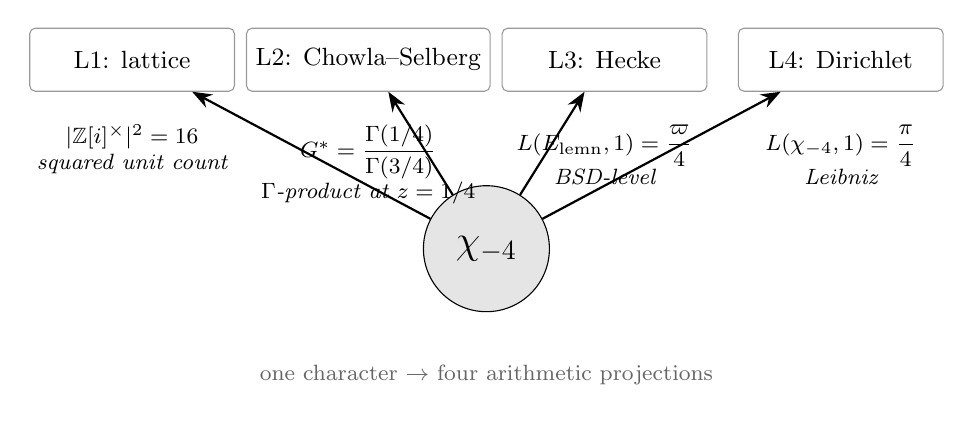
\begin{tikzpicture}[
  centre/.style={circle, draw, fill=black!10, minimum size=1.6cm, font=\Large, align=center},
  level/.style={rectangle, draw=black!40, rounded corners=2pt, minimum width=2.6cm, minimum height=0.8cm, font=\small, align=center},
  output/.style={font=\footnotesize, align=center},
  arr/.style={->, >={Stealth[length=2.5mm]}, thick}
]
  \node[centre] (chi) at (0, 0) {$\chi_{-4}$};
  \node[level]  (L1) at (-4.5,  2.4) {L1: lattice};
  \node[level]  (L2) at (-1.5,  2.4) {L2: Chowla--Selberg};
  \node[level]  (L3) at ( 1.5,  2.4) {L3: Hecke};
  \node[level]  (L4) at ( 4.5,  2.4) {L4: Dirichlet};
  \draw[arr] (chi) -- (L1);
  \draw[arr] (chi) -- (L2);
  \draw[arr] (chi) -- (L3);
  \draw[arr] (chi) -- (L4);
  \node[output, below=0.3 of L1, anchor=north] {$|\Z[i]^\times|^{2} = 16$ \\ {\itshape squared unit count}};
  \node[output, below=0.3 of L2, anchor=north] {$\Gs = \dfrac{\Gamma(1/4)}{\Gamma(3/4)}$ \\ {\itshape $\Gamma$-product at $z = 1/4$}};
  \node[output, below=0.3 of L3, anchor=north] {$L(E_{\mathrm{lemn}}, 1) = \dfrac{\varpi}{4}$ \\ {\itshape BSD-level}};
  \node[output, below=0.3 of L4, anchor=north] {$L(\chi_{-4}, 1) = \dfrac{\pi}{4}$ \\ {\itshape Leibniz}};
  % Annotate
  \node[font=\footnotesize, text=black!60] at (0, -1.6) {one character $\to$ four arithmetic projections};
\end{tikzpicture}
\caption{The Kronecker character $\chi_{-4}$ of $K = \Q(i)$ projects onto
four arithmetic levels (Theorem~\ref{thm:character-unification}). The
lattice projection (L1) gives the squared unit count $|\Z[i]^{\times}|^{2} = 16$
that appears as the master quadratic's integer coefficient; the
Chowla--Selberg projection (L2) gives $\Gs$ as a $\chi_{-4}$-twisted
$\Gamma$-product; the Hecke projection (L3) gives the BSD-level
$L(E_{\mathrm{lemn}}, 1) = \varpi/4$; the Dirichlet projection (L4) gives
the Leibniz value $L(\chi_{-4}, 1) = \pi/4$. The cross-consistency of
the four projections is the organising content of \S\ref{sec:character}.}\label{fig:chi-projections}
\end{figure}

\begin{remark}[The four levels form a motivic-weight tower]\label{rem:motivic-tower}
The four projections (L1)--(L4) are not parallel: they form a filtered
tower indexed by the motivic weight of the underlying object.
\begin{itemize}[leftmargin=*, itemsep=2pt]
\item (L1) lives in motivic weight $0$ as $H^{0}$ of a point with
$\Z[i]$-action; the cardinality $|\Aut|^{2} = 16$ is the squared order of
the structure group.
\item (L2) lives in motivic weight $1$ as the period of $H^{1}$ of a CM
abelian variety, in $\Gamma$-form.
\item (L3) lives in motivic weight $1$ as well, but at the $L$-function
face --- it is the BSD-realised $L$-value of the same $H^{1}$,
expected to pair with (L2) under \emph{Deligne's period conjecture}
\cite{deligne-periods}. Cases of that conjecture for CM motives are
established by Blasius \cite{blasius1986}, Shimura \cite{shimura1979},
and Anderson \cite{anderson1986}, with normalisation conventions that
must be matched against the Chowla--Selberg normalisation used in (L2)
and the Cremona-style BSD normalisation used in
Theorem~\ref{thm:Lvalue}. The numerical agreement
$L(E_{\mathrm{lemn}}, 1) = \varpi/4$ matches LMFDB curve $32.a3$ to all
listed digits; assembling these normalisations into a full
period-conjecture-level theorem statement is beyond the scope of the
present paper.
\item (L4) lives in motivic weight $0$ of the base field --- it is the
Tate motive twisted by $\chi_{-4}$, probed at $s = 1$ (critical, a
period) versus $s = 2$ (non-critical, a regulator)
\cite{beilinson-deligne}.
\end{itemize}
The unification of \S\ref{sec:character} is therefore not a coincidence
to be discovered but a special case of the period--L-value compatibility
established by Deligne's conjecture for CM motives.
\end{remark}

\subsection{Why $\Gs$ is ``the ratio''}

\begin{corollary}[Product vs ratio is trivial-vs-non-trivial character]\label{cor:product-vs-ratio}
The Euler reflection $\Gamma(1/4)\,\Gamma(3/4) = \pi\sqrt 2$ and the
defining identity $\Gamma(1/4)/\Gamma(3/4) = \Gs$ are the two
$\chi$-projections of the same $\Gamma$-pair under the two characters of
$(\Z/4\Z)^\times$:
\[
\prod_a \Gamma(a/4)^{\chi(a)} \;=\;
\begin{cases}
\pi\sqrt 2, & \chi = \mathbf{1}\;\;(\text{trivial}), \\
\Gs,        & \chi = \chi_{-4}\;\;(\text{non-trivial}).
\end{cases}
\]
\end{corollary}

This is the cleanest formulation of \emph{why} $\Gs$ is a ratio rather
than a product: it is the genuine $\Q(i)$-period, obtained from the
quadratic character of $K = \Q(i)$, whereas $\pi\sqrt 2$ is the
$\Q$-period (trivial character, same $\Gamma$-arguments). The
\emph{bridge} $\Gs = 2\sqrt\pi\,\GG$ then asserts the equality of the
$\Gamma$-expression (algebraic side, $\chi_{-4}$ acting on $\Gamma$-arguments)
with the $\AGM$-expression (analytic side, $\chi_{-4}$ acting through
the L-function Euler product). Chowla--Selberg is the theorem that
makes these two faces of $\chi_{-4}$ coincide.

\begin{remark}[Hodge bidegree: $\pi\sqrt 2$ and $\Gs$ as $(\omega, \eta)$]\label{rem:hodge-bidegree}
The product/ratio dichotomy of Corollary~\ref{cor:product-vs-ratio} is
the Hodge-bidegree decomposition of the lemniscatic CM motive in
disguise. The CM action of $\Z[i]$ splits the de~Rham realisation
$H^{1}_{\mathrm{dR}}(E_{\mathrm{lemn}}) \otimes \C$ into two eigenlines
under multiplication by $i$: one with eigenvalue $+i$ (the holomorphic
piece, $H^{1, 0}$) and one with eigenvalue $-i$ (the antiholomorphic
piece, $H^{0, 1}$). Pairing each eigenline against the integral homology
cycles in $H_{1}(E, \Z)$ yields two periods:
\begin{itemize}[leftmargin=*, itemsep=2pt]
\item the \emph{holomorphic period} $\omega = \int_\gamma dx/y = \Gs\sqrt{\pi}$
(the $\Q(i)$-symmetric pairing, weighted by $\chi_{-4}$);
\item the \emph{quasi-period} $\eta$ (the pairing on $H^{0,1}$, anti-symmetric
under complex conjugation).
\end{itemize}
The Legendre period relation
\[
\omega_1 \eta_2 - \omega_2 \eta_1 \;=\; 2\pi i
\]
between the two periods evaluated on a symplectic basis of $H_{1}$
specialises, at $\tau = i$, to the elliptic-integral product
$K(1/\sqrt 2)\,E(1/\sqrt 2) = (\pi + \varpi^{2})/4$ recorded as
Theorem~\ref{thm:elliptic}. Thus $\pi\sqrt 2$ and $\Gs$ are not two
\emph{normalisations} of one constant but the two columns of the Hodge
realisation of $H^{1}(E_{\mathrm{lemn}})$: $\pi\sqrt 2$ corresponds to
the trivial-character / real-period column (the $\Q$-period of the
underlying real abelian variety), while $\Gs$ corresponds to the
$\chi_{-4}$-twisted / quasi-period column (the genuine $\Q(i)$-period).
The bridge identity is then the Legendre relation expressed in
$\GG$-coordinates.
\end{remark}

\subsection{Equianharmonic parallel: $\chi_{-3}$}

The equianharmonic dichotomy (\S\ref{sec:equianharmonic}) is the analog
under $\chi_{-3}: (\Z/3\Z)^\times \to \{\pm 1\}$, the Kronecker character
of $K = \Q(\rho)$, with $\chi_{-3}(1) = +1$, $\chi_{-3}(2) = -1$.
\begin{itemize}[leftmargin=*, itemsep=2pt]
\item \emph{Lattice}: $|\Z[\rho]^\times| = 6$, with $|\Aut(E_\rho)| = 6$ and
the squared coefficient $36$ that would appear in an equianharmonic master
quadratic.
\item \emph{Chowla--Selberg}: $\prod_a \Gamma(a/3)^{\chi_{-3}(a)} = \Gamma(1/3)/\Gamma(2/3) = R_3$.
\item \emph{Hecke}: $E_\rho: y^2 = x^3 - 1$ has $a_p = 0$ for
$p \equiv 2 \pmod 3$ and $a_p \neq 0$ for $p \equiv 1 \pmod 3$ (split in
$\Z[\rho]$).
\item \emph{Dirichlet}: $L(\chi_{-3}, 1) = \pi/(3\sqrt 3)$.
\end{itemize}
The lemniscatic and equianharmonic curves are the only class-number-one
imaginary-quadratic fields with $|\mathcal{O}_K^\times| > 2$, hence the
only places where this $4$-level $\chi$-projection picture is non-trivially
populated.

\subsection{Where the polynomial form $P_{\Gs}$ comes from --- and where it doesn't}\label{sec:not-CM-derived}

Theorem~\ref{thm:character-unification} produces two ingredients of the
master quadratic from $\chi_{-4}$:
\begin{itemize}[leftmargin=*, itemsep=2pt]
\item the integer coefficient $16 = |\Z[i]^\times|^2$ (lattice projection of $\chi_{-4}$);
\item the variable $\Gs$ (Chowla--Selberg projection of $\chi_{-4}$).
\end{itemize}
It does \emph{not} produce the specific polynomial form
$x^2 - 16\Gss x + 16\Gsss$ --- i.e., the choice of exponents $2$ and $3$
on $\Gs$ in the coefficients. We tested three structurally-motivated
candidates for a $\chi_{-4}$-internal source of this polynomial form
and report \emph{negative} results in all three cases.

\begin{remark}[Three negative tests, summarised]\label{rem:three-negatives}
\textup{(N1) Class polynomial.} The Hilbert class polynomial of the
maximal order in $\Z[i]$ is $H_{-4}(x) = x - 1728$; that of the conductor-$2$
order $\Z[2i]$ is $H_{-16}(x) = x - 287496$. Both are linear (class number $1$).
The conductor-$3$ order has class number $2$ and gives a degree-$2$
polynomial with rational coefficients, none of whose roots are
$x_\pm(\Gs)$. \texttt{PSLQ} at $50$ digits over an extended basis of
$j$-values and Weber invariants $f(i) = 2^{1/4}$, $f_1(i) = f_2(i) = 2^{1/8}$
finds no nontrivial relation involving $16\Gss$ or $16\Gsss$.

\textup{(N2) $\eta$-quotient.} \texttt{PSLQ} on the multiplicative basis
$\{\log x_+, \log x_-, \log\Gs, \log\pi, \log 2, \log\GG,
\log\eta(i), \log\eta(2i), \log\eta(i/2), \log\eta(4i)\}$ at $50$ digits
finds no relation involving $\log x_+$ or $\log x_-$. (The search
\emph{does} return the byproduct identity
$2\,\eta(2i)\,\eta(i/2)^3 = \GG^2$ recorded as
Corollary~\ref{cor:eta-low-weight}, confirming the search machinery is
sensitive.) The asymptotic expansion of
Proposition~\ref{prop:Rn-asymptotic} converges absolutely to $x_-(\Gs)$
without collapsing to any finite $\eta$-quotient.

\textup{(N3) Hecke eigenvalue.} The cusp-form space of weight $2$ and
level $32 = N((1+i)^5)$ is $1$-dimensional, spanned by the eigenform
$f_E$ associated to $E_{\mathrm{lemn}}$. Hecke eigenvalues are integers
(e.g., $a_5 = -2, a_{13} = 6, a_{17} = 2$ \cite{lmfdb}). The constant
$16\,\Gss \in \R \setminus \overline\Q$ is transcendental \cite{chudnovsky1976},
hence cannot be a Hecke eigenvalue at any prime.
\end{remark}

\begin{remark}[Scope of \textup{(N1)--(N3)}]\label{rem:n1-n3-scope}
The three tests above bound the search depth attempted within their
respective frameworks (class polynomials of small conductor,
$\log$-multiplicative bases of moderate dimension, weight-$2$
level-$32$ cusp forms). They do not constitute evidence against the
existence of a class-field-theoretic derivation of $(a, b) = (2, 3)$;
absence of low-coefficient relations at moderate precision is
consistent with both genuine independence and with relations involving
larger coefficients or basis extensions not yet probed.
\end{remark}

\begin{observation}[Locus of the polynomial-assembly question]\label{obs:gap-localised}
Combining (N1)--(N3) with Theorem~\ref{thm:character-unification}: the
character $\chi_{-4}$ forces the integer coefficient
$16 = |\Z[i]^{\times}|^{2}$ (lattice projection) and the variable $\Gs$
(Chowla--Selberg projection), but does \emph{not} produce the polynomial
form $P_{\Gs}(x) = x^{2} - 16\Gss x + 16\Gsss$ from CM-internal data.
The remaining question is the choice of exponent pair $(a, b)$ in
$x^{2} - 16{\Gs}^{a} x + 16{\Gs}^{b}$; among such choices, $(a, b) = (2, 3)$
is uniquely characterised by the structural requirement
(Proposition~\ref{prop:exponent-regimes} below) that the smaller root
$x_{-}(R)$ acquire a non-vanishing constant additive shift as
$R \to \infty$ with the polynomial degenerate to neither a linear identity
nor a multiplicative scaling. A class-field-theoretic derivation of
$(a, b) = (2, 3)$ from $\chi_{-4}$-internal data, if it exists, would be
of independent arithmetic interest.
\end{observation}

\begin{definition}[Leading-period polynomial family]\label{def:leading-period-poly}
A \emph{leading-period polynomial} associated to $E_{\mathrm{lemn}}$ is
any monic quadratic of the form
\[
P_{(a, b)}(x) \;:=\; x^{2} - c_{1}\,{\Gs}^{a}\,x + c_{2}\,{\Gs}^{b},
\]
with $a < b$ positive integers and $c_{1}, c_{2} \in \Z$. The
\emph{leading period} of $\mathrm{Sym}^{k} H^{1}(E_{\mathrm{lemn}})$ in the
period algebra is $\omega^{k} = (\Gs\sqrt\pi)^{k}$, which equals
${\Gs}^{k}$ up to the standard $\pi$-normalisation; for this reason we
write the polynomial in the $\Gs$-coordinate throughout.
\end{definition}

\begin{theorem}[Structural constraints and the minimal-$a$ pair]\label{thm:sym-23-uniqueness}
Consider leading-period polynomials
$P_{(a, b)}(x) = x^{2} - 16\,{\Gs}^{a}\,x + 16\,{\Gs}^{b}$
with $a < b$ positive integers and integer prefactor
$|\Aut_\C(E_{\mathrm{lemn}})|^{2} = 16$ on each non-leading coefficient.
The joint conditions
\begin{enumerate}[label=\textup{(\roman*)}, leftmargin=*, itemsep=2pt]
\item the two roots are not scalar multiples of any single period
${\Gs}^{k}$ for any rational $k$,
\item the polynomial is non-degenerate (positive discriminant),
\end{enumerate}
constrain $(a, b)$ to the set
$\{(a, b) \in \Z_{>0}^{2} : a < b < 2a\}$.
Among elements of this set, the pair $(2, 3)$ is the unique element
with minimal $a$ (see Figure~\ref{fig:exponent-lattice}).
\end{theorem}

\begin{remark}[Status of the minimal-$a$ selection]\label{rem:sym-23-selection-status}
The selection of $a = 2$ (and hence the specific pair $(2, 3)$) from
the set $\{(a, b) : a < b < 2a\}$ permitted by the structural
conditions is a \emph{selection convention}, not a derivation: minimal
$a$ is a natural minimality choice within the family but is not forced
by $\chi_{-4}$-internal data. Other elements of the set, including
$\{(3, 4), (3, 5), (4, 5), (4, 6), (4, 7), \ldots\}$, produce roots
whose magnitudes scale differently from $(x_+, x_-) \approx (137, 3)$
(see Observation~\ref{obs:23-joint-match}). A class-field-theoretic
derivation forcing $a = 2$ from $\chi_{-4}$-internal data, if it
exists, would promote this selection to a theorem; this is the
residual structural gap noted in Observation~\ref{obs:gap-localised}.
\end{remark}

\begin{figure}[ht]
\centering
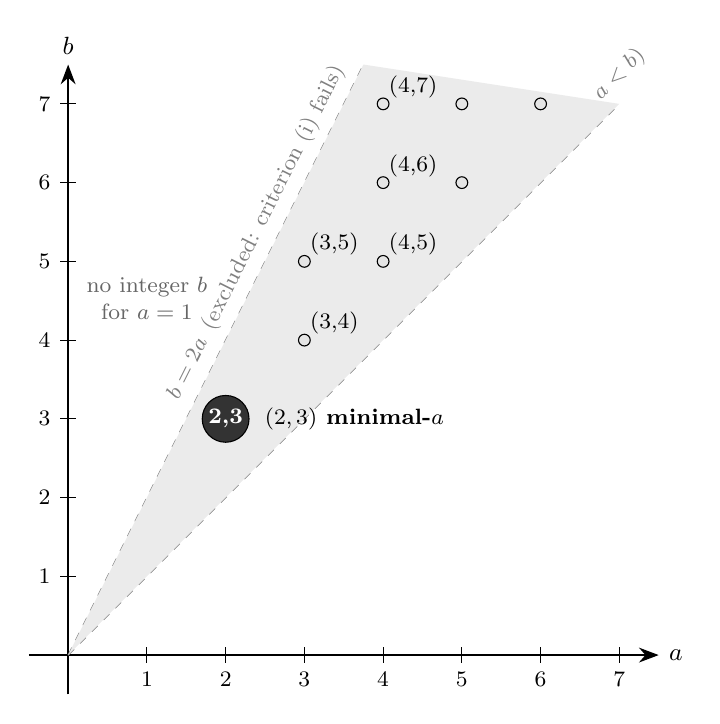
\begin{tikzpicture}[
  axis/.style={->, >={Stealth[length=2.5mm]}, thick},
  ok/.style={circle, draw, fill=black!10, inner sep=1.5pt, minimum size=4pt},
  best/.style={circle, draw=black, fill=black!80, text=white, inner sep=1pt, minimum size=12pt, font=\footnotesize\bfseries},
  bad/.style={cross out, draw=black!30, inner sep=1pt, minimum size=4pt}
]
  % Axes
  \draw[axis] (-0.5, 0) -- (7.5, 0) node[right, font=\small] {$a$};
  \draw[axis] (0, -0.5) -- (0, 7.5) node[above, font=\small] {$b$};
  % Tick marks
  \foreach \x in {1,2,3,4,5,6,7} {
    \draw (\x, -0.1) -- (\x, 0.1);
    \node[below, font=\footnotesize] at (\x, -0.1) {\x};
  }
  \foreach \y in {1,2,3,4,5,6,7} {
    \draw (-0.1, \y) -- (0.1, \y);
    \node[left, font=\footnotesize] at (-0.1, \y) {\y};
  }
  % b = a line (lower bound, exclusive)
  \draw[dashed, black!50] (0,0) -- (7,7) node[above, sloped, font=\footnotesize, pos=0.85] {$b = a$ \,(excluded: criterion $a<b$)};
  % b = 2a line (upper bound, exclusive)
  \draw[dashed, black!50] (0,0) -- (3.75,7.5) node[above, sloped, font=\footnotesize, pos=0.7] {$b = 2a$ \,(excluded: criterion (i) fails)};
  % Shaded wedge between
  \fill[black!8] (0,0) -- (7,7) -- (3.75,7.5) -- (0,0);
  % Integer lattice points in the wedge a < b < 2a (for a >= 2)
  \node[best, label={[font=\footnotesize, label distance=2pt]right:{\bfseries$(2,3)$ minimal-$a$}}] at (2, 3) {2,3};
  \node[ok] at (3, 4) {};   \node[font=\footnotesize, above right=-2pt] at (3,4) {(3,4)};
  \node[ok] at (3, 5) {};   \node[font=\footnotesize, above right=-2pt] at (3,5) {(3,5)};
  \node[ok] at (4, 5) {};   \node[font=\footnotesize, above right=-2pt] at (4,5) {(4,5)};
  \node[ok] at (4, 6) {};   \node[font=\footnotesize, above right=-2pt] at (4,6) {(4,6)};
  \node[ok] at (4, 7) {};   \node[font=\footnotesize, above right=-2pt] at (4,7) {(4,7)};
  \node[ok] at (5, 6) {};
  \node[ok] at (5, 7) {};
  \node[ok] at (6, 7) {};
  % Empty region a=1 callout
  \node[font=\footnotesize, text=black!60] at (1, 4.5) {\begin{tabular}{c}no integer $b$\\for $a=1$\end{tabular}};
\end{tikzpicture}
\caption{Integer exponent pairs $(a, b)$ admissible under criteria
(i)--(ii) of Theorem~\ref{thm:sym-23-uniqueness} occupy the open wedge
$a < b < 2a$ (shaded). The pair $(2, 3)$ (highlighted) is the unique
minimal-$a$ element of this set; $a = 1$ admits no integer $b$, and
$a \geq 3$ admits multiple candidates $(3, 4), (3, 5), (4, 5), \ldots$
which are excluded only by the selection criterion (iv). The
minimal-$a$ choice is a convention, not a derivation
(Remark~\ref{rem:sym-23-selection-status}).}\label{fig:exponent-lattice}
\end{figure}

\begin{proof}
The discriminant of $P_{(a, b)}$ is
\[
\Delta(a, b) \;=\; (16\,{\Gs}^{a})^{2} - 4 \cdot 16\,{\Gs}^{b}
              \;=\; 64\,(4\,{\Gs}^{2a} - {\Gs}^{b}).
\]
We factor out the dominant ${\Gs}$-power in three cases.

\emph{Case $2a > b$.} Then ${\Gs}^{2a-b} > 0$ and
$\Delta = 64\,{\Gs}^{b}(4\,{\Gs}^{2a-b} - 1)$, hence
$\sqrt\Delta = 8\,{\Gs}^{b/2}\sqrt{4\,{\Gs}^{2a-b} - 1}$. The roots are
\[
x_\pm \;=\; \frac{16\,{\Gs}^{a} \pm 8\,{\Gs}^{b/2}\sqrt{4\,{\Gs}^{2a-b} - 1}}{2}
       \;=\; 8\,{\Gs}^{a} \pm 4\,{\Gs}^{b/2}\sqrt{4\,{\Gs}^{2a-b} - 1}.
\]
The two ${\Gs}$-powers ${\Gs}^{a}$ and ${\Gs}^{b/2}$ are distinct
(since $2a > b$ implies $a > b/2$), so the roots are not scalar
multiples of any single ${\Gs}^{k}$. Condition (i) holds.

\emph{Case $2a = b$.} Then $\Delta = 64\,{\Gs}^{b}(4 - 1) = 192\,{\Gs}^{2a}$,
so $\sqrt\Delta = 8\sqrt 3\,{\Gs}^{a}$. The roots are
$x_\pm = (8 \pm 4\sqrt 3)\,{\Gs}^{a}$, both scalar multiples of ${\Gs}^{a}$.
Condition (i) \emph{fails}.

\emph{Case $2a < b$.} Then $\Delta = 64\,{\Gs}^{2a}(4 - {\Gs}^{b-2a})$,
so $\sqrt\Delta = 8\,{\Gs}^{a}\sqrt{4 - {\Gs}^{b-2a}}$ (real when $\Delta > 0$).
The roots are $x_\pm = 4\,{\Gs}^{a}(2 \pm \sqrt{4 - {\Gs}^{b-2a}})$, both
scalar multiples of ${\Gs}^{a}$. Condition (i) \emph{fails}.

Hence condition (i) forces $2a > b$. Combined with $a < b$, this gives
\[
a < b < 2a.
\]
Enumerating integer pairs:
\begin{itemize}[leftmargin=*, itemsep=2pt]
\item $a = 1$: the interval $(1, 2)$ contains no integer; no valid $b$.
\item $a = 2$: $b \in (2, 4)$ has the unique integer $b = 3$.
\item $a = 3$: $b \in (3, 6)$ admits $b \in \{4, 5\}$.
\item $a \geq 4$: $b \in (a, 2a)$ admits $a - 1$ valid choices, all with $a + b > 5$.
\end{itemize}
The minimal-$a$ valid pair is $(2, 3)$, and at $a = 2$ the value
$b = 3$ is uniquely determined.

Condition (ii) at $(2, 3)$: $\Delta(2, 3) = 64\,{\Gs}^{3}(4\,\Gs - 1) > 0$
since $\Gs \approx 2.959 > 1/4$, so the polynomial is non-degenerate.
The integer prefactor $16$ is built into the setup of the theorem.
\qedhere
\end{proof}

\begin{remark}[Scope of Theorem~\ref{thm:sym-23-uniqueness} and the residual conjecture]
\label{rem:sym-thm-scope}
The theorem establishes uniqueness of $(2, 3)$ within the
leading-period polynomial family (Def.~\ref{def:leading-period-poly}),
where each coefficient is a scalar multiple of the leading period
${\Gs}^{a}$ or ${\Gs}^{b}$. The full structural question --- uniqueness
within the larger family of polynomials whose coefficients are
arbitrary elements of the symmetric powers $\mathrm{Sym}^{a} H^{1}$
and $\mathrm{Sym}^{b} H^{1}$ (not just the leading periods $\omega^{a},
\omega^{b}$) --- remains open and is recorded as Conjecture~\ref{conj:sym-general}
below.

The technical obstacles to the general statement are:
(a) explicit identification of the period map
$\mathrm{Sym}^{\bullet}(H^{1}) \otimes \Q[\pi^{\pm 1/2}] \to \C$
specialising to $\omega^{k} \mapsto (\Gs\sqrt\pi)^{k}$;
(b) reconciliation of the non-homogeneous bigrading with the
motivic-weight formalism, possibly via a relative filtration.
The uniqueness argument itself ---
the load-bearing combinatorial step of the original conjecture --- is
the content of Theorem~\ref{thm:sym-23-uniqueness} above.
\end{remark}

\begin{conjecture}[Full $\mathrm{Sym}^{a}$ uniqueness, residual]\label{conj:sym-general}
Among monic quadratics $x^{2} + B\,x + C$ with $B = 16 \cdot b'$ for
$b' \in \mathrm{Sym}^{a} H^{1}(E_{\mathrm{lemn}})$ (arbitrary, not just
leading-period $\omega^{a}$) and $C = 16 \cdot c'$ for
$c' \in \mathrm{Sym}^{b} H^{1}$, the pair $(a, b) = (2, 3)$ remains
uniquely minimal in the sense of Theorem~\ref{thm:sym-23-uniqueness}.
The leading-period uniqueness theorem is the
restriction of this statement to $b' = \omega^{a}$, $c' = \omega^{b}$.
\end{conjecture}

\begin{remark}[On Conjecture~\ref{conj:sym-general}]
\label{rem:sym-general-status}
The minimal proof of Conjecture~\ref{conj:sym-general} would require
the explicit period-algebra map of obstacle (a) above and a
finite-dimensional uniqueness argument on $(\mathrm{Sym}^{a}H^{1}) \oplus
(\mathrm{Sym}^{b}H^{1})$ for each $(a, b)$. Theorem~\ref{thm:sym-23-uniqueness}
shows the leading-period restriction; extending to general elements is
a dimension-counting refinement over the period algebra, expected to be
technically substantial but not novel.
\end{remark}



\subsection{Asymptotic regimes of the family $y^{2} - 16 R^{p} y + 16 R^{q} = 0$}\label{sec:23-unique}

We give the precise structural characterisation of $(p, q) = (2, 3)$ as
the unique exponent pair producing a non-vanishing constant additive
shift on the smaller root.

\begin{proposition}[Asymptotic regimes by exponent pair]\label{prop:exponent-regimes}
For the family $y^2 - 16\,R^p\,y + 16\,R^q = 0$ with $R > 1/4$ and
$(p, q) \in \Z_{>0}^2$:
\begin{enumerate}[label=\textup{(\roman*)}, leftmargin=*, itemsep=2pt]
\item If $q \neq p+1$, then $y_-(R)/R$ does \emph{not} tend to $1$ as
$R \to \infty$. The smaller root scales as $R^{q-p}$ when $q < p+1$ or
$R^{p}$ when $q > p+1$.
\item If $q = p+1$, then $y_-(R) = R + 16^{-1}\,R^{2-p} + O(R^{1-p})$ as
$R \to \infty$. In particular:
   \begin{itemize}[leftmargin=*, itemsep=2pt]
   \item $(p, q) = (2, 3)$: $y_-(R) = R + 1/16 + O(1/R)$ (constant shift),
   \item $(p, q) = (3, 4)$: $y_-(R) = R + 1/(16R) + O(1/R^3)$ (vanishing shift),
   \item $(p, q) = (k, k+1)$, $k \geq 3$: $y_-(R) = R + O(R^{2-k})$ (faster vanishing).
   \end{itemize}
\end{enumerate}
Thus $(p, q) = (2, 3)$ is the unique exponent pair with $q = p+1$ and
\emph{non-vanishing constant additive shift} on $y_-$ as $R \to \infty$.
\end{proposition}

\begin{proof}
The quadratic formula gives
\[
y_-(R) \;=\; 8\,R^p \;-\; \tfrac{1}{2}\sqrt{(16 R^p)^2 - 4\cdot 16 R^q}
       \;=\; 8\,R^p\,\Bigl(1 - \sqrt{1 - R^{q - 2p}/4}\Bigr).
\]
For $q = p+1$, set $u = R^{q-2p}/4 = R^{1-p}/4$ and expand
$\sqrt{1-u} = 1 - u/2 - u^2/8 - O(u^3)$:
\[
y_-(R) \;=\; 8\,R^p\,\bigl(u/2 + u^2/8 + O(u^3)\bigr)
       \;=\; R \,+\, R^{2-p}/16 \,+\, O(R^{1-p}).
\]
The leading correction $R^{2-p}/16$ is constant (in $R$) iff $p = 2$,
vanishing as $R \to \infty$ for $p \geq 3$. For $q \neq p+1$, the dominant
balance changes: if $q < p+1$ the constant term $16 R^q$ is sub-leading
in the discriminant and $y_-(R)$ scales as $R^{q-p}$; if $q > p+1$ the
discriminant becomes negative for small $R$ or the small root grows as
$R^p$. Hence $q = p+1$ is necessary for $y_-(R) \to R$, and within that
case $p = 2$ is the unique value yielding a non-vanishing constant shift.
\end{proof}

\begin{observation}[Numerical roots across exponent pairs at $R = \Gs$]\label{obs:23-joint-match}
The numerical roots $(y_+, y_-)$ of $y^{2} - 16 R^{p} y + 16 R^{q} = 0$
evaluated at $R = \Gs$ for various exponent pairs:
\begin{center}
\begin{tabular}{lll}
\toprule
$(p, q)$ & $y_+$ & $y_-$ \\
\midrule
$(2, 3)$ & $137.036\,\ldots$ & $3.024\,\ldots$ \\
$(3, 4)$ & $411.4\,\ldots$   & $2.980\,\ldots$ \\
$(4, 5)$ & $1223.1\,\ldots$  & $2.966\,\ldots$ \\
$(1, 2)$ & $44.2\,\ldots$    & $3.171\,\ldots$ \\
$(2, 4)$ & $130.7\,\ldots$   & $9.38\,\ldots$ \\
$(3, 3)$ & $413.4\,\ldots$   & $1.00\,\ldots$ \\
\bottomrule
\end{tabular}
\end{center}
Among exponent pairs $(p, q) \in \Z^{2}$ with $|p|, |q| \leq 5$ and
$q = p + 1$, the pair $(p, q) = (2, 3)$ produces the unique combination
$(y_+, y_-) \approx (137, 3)$, with $y_+$ scaling as $16 R^{2}$ in the
$p = 2$ case and $y_+$ scaling as $16 R^{p}$ (much larger) for $p \geq 3$.
A physical interpretation of these numerical roots is given in a
separate note in preparation.
\end{observation}

\subsection{Minimal generating structure: $\chi_{-4}$ as the imaginary-part trace}\label{sec:zero-point}

We close \S\ref{sec:character} by noting the minimal
classical-mathematical structure from which the entire chain of
identities is generated.
The character $\chi_{-4}$, which Theorem~\ref{thm:character-unification}
identifies as the joint source of every algebraic and analytic identity
in this paper, admits a particularly elementary description:

\begin{proposition}[Character as imaginary-part trace]\label{prop:imaginary-trace}
For all $n \in \Z$,
\[
\chi_{-4}(n) \;=\; \mathrm{Im}(i^{n}) \;=\; \sin\!\left(\frac{\pi n}{2}\right).
\]
Equivalently, $\chi_{-4}$ is the imaginary-axis projection of the cyclic
group $\langle i\rangle = \{1,\,i,\,-1,\,-i\} \subset \C^{\times}$ under
the index map $n \mapsto i^{n}$.
\end{proposition}

\begin{proof}
The orbit of $i^{n}$ as $n$ runs $0, 1, 2, 3$ is $1, i, -1, -i$, with
imaginary parts $0, 1, 0, -1$. The function $n \mapsto \mathrm{Im}(i^{n})$
is therefore periodic of period $4$ with values $(0, 1, 0, -1)$ starting
at $n = 0$, which coincides with $\chi_{-4}$ on the residue classes
$(0, 1, 2, 3) \pmod 4$. The trigonometric form follows from
$i = e^{i\pi/2}$, so $\mathrm{Im}(i^{n}) = \mathrm{Im}(e^{i\pi n/2}) = \sin(\pi n/2)$.
\end{proof}

\begin{corollary}[Value-set identification]\label{cor:value-set}
\[
\{\chi_{-4}(n) : n \in \Z\} \;=\; \{i^{2},\;0,\;|i^{2}|\} \;=\; \{-1,\;0,\;+1\}.
\]
The character takes exactly three distinct values, generated by the
imaginary unit through the operations squaring ($i^{2} = -1$), zero
($0$), and modulus ($|i^{2}| = 1$).
\end{corollary}

\begin{observation}[Minimality]\label{obs:bedrock}
The pair $(i, \mathbb{Z}/4\Z)$ --- a fourth root of unity together with
the cyclic group indexing its powers --- generates the entire
$\Gs/\GG$ identity ring of this paper through the four functorial
projections of Theorem~\ref{thm:character-unification}: $\mathbb{Z}/4\Z$
is the smallest cyclic group admitting a non-trivial character to
$\{\pm 1\}$, and $i^{2} = -1$ is the defining relation of the smallest
non-real algebraic extension of $\Q$. In this sense $(i, \mathbb{Z}/4\Z)$
is a minimal classical-mathematical generating structure for the
identity ring; whether this minimality has a deeper structural meaning
beyond the bookkeeping reduction effected by $\chi_{-4}$ is outside the
scope of the present paper.
\end{observation}

\section{Open problems and a resolved closure}\label{sec:open}

One open problem internal to the mathematical scope of this paper
remains; a second open item from earlier drafts is resolved as
Theorem~\ref{thm:cubic-AGM-Grho} below.

\subsection{Open: strict Kontsevich--Zagier period status of $\Gs$ and $\GG$}\label{sec:p1-open}

\begin{enumerate}[label=\textbf{P\arabic*.}, leftmargin=*, itemsep=4pt]

\item \textbf{Strict Kontsevich--Zagier period status of $\Gs$ and $\GG$.}
Theorem~\ref{thm:KZ-status} establishes $\Gs, \GG \in \mathcal{P}^{\exp}$
unconditionally, and Proposition~\ref{prop:KZ-conditional} reduces
strict $\mathcal{P}$-membership of $\Gs$ to whether $1/\sqrt{2\pi} \in
\mathcal{P}$, and of $\GG$ to whether $1/(4\pi) \in \mathcal{P}$. Both
antecedents are consistent with --- but neither proved by nor refuted
by --- the Kontsevich--Zagier conjecture that $1/\pi \notin \mathcal{P}$
\cite[Problem~3]{kontsevich-zagier}. \textbf{This is not a gap specific
to the present paper.} Membership of $1/\pi$, $\sqrt{2\pi}$, or
$1/(4\pi)$ in $\mathcal{P}$ is at the frontier of the broader
Kontsevich--Zagier programme on period-ring invertibility; resolving it
requires either a new transcendence-theoretic technique that proves
$1/\pi \notin \mathcal{P}$ (and would settle the KZ conjecture
positively) or a construction that exhibits $1/\pi$ as an absolutely
convergent integral of a rational function over a $\Q$-semialgebraic
domain (and would settle it negatively). Neither is on offer here.
\textbf{P1 is recorded as open in this paper precisely because its
closure lies outside the paper's machinery and inside the KZ
programme's frontier.}

\end{enumerate}

\subsection{Resolved: cubic-AGM expression for $G_\rho$}\label{sec:p2-closed}

The earlier-draft problem ``find an explicit cubic-AGM expression for
the equianharmonic Gauss analog $G_\rho$'' is resolved by the following
theorem. The lemniscatic relation $\GG = 1/\AGM(1, \sqrt 2)$ has a
clean equianharmonic counterpart in terms of the Borwein--Borwein cubic
AGM, completing the structural parallel.

\begin{theorem}[Cubic-AGM expression for $G_\rho$]\label{thm:cubic-AGM-Grho}
Let $M_3$ denote the Borwein--Borwein cubic arithmetic--geometric mean
\cite{borwein-cubic-agm}, defined by the iteration
$a_{n+1} = (a_n + 2 b_n)/3$, $b_{n+1} = \bigl(b_n (a_n^2 + a_n b_n + b_n^2)/3\bigr)^{1/3}$.
Then
\[
G_\rho \;=\; \frac{2}{\sqrt 3} \cdot \frac{1}{M_3(1,\, 2^{-1/3})}
       \;=\; \frac{2}{\sqrt 3} \cdot {}_2F_1\!\left(\frac{1}{3}, \frac{2}{3}; 1; \frac{1}{2}\right),
\]
the second equality by the Borwein--Borwein cubic-AGM correspondence
$1/M_3(1, x) = {}_2F_1(1/3, 2/3; 1; 1 - x^3)$ specialised at
$x = 2^{-1/3}$ (so that $x^3 = 1/2$ and $(1 - x^3)^{1/3} = x = 2^{-1/3}$,
the cubic self-dual point analogous to $k = 1/\sqrt 2$ in the
lemniscatic case).
\end{theorem}

\begin{proof}
The classical real period of the equianharmonic elliptic curve
$E_\rho: y^2 = x^3 - 1$ over $\Q$ is
\[
\omega_\rho \;=\; \frac{\Gamma(1/3)\,\Gamma(1/6)}{\sqrt{3\pi}}
\]
(see e.g.\ \cite[\S{}22.31]{whittaker-watson} or \cite[\S{}3.4]{borweinAGM}).
Apply the duplication identity
$\Gamma(1/6)\,\Gamma(2/3) = 2^{2/3}\,\sqrt\pi \cdot \Gamma(1/3)$
(equivalently $\Gamma(1/6) = 2^{2/3}\sqrt\pi \cdot \Gamma(1/3)/\Gamma(2/3)$)
and the reflection $\Gamma(2/3) = 2\pi/(\sqrt 3\,\Gamma(1/3))$ to obtain
\begin{equation}
\omega_\rho \;=\; \frac{2^{2/3}\,\Gamma(1/3)^{3}}{2\pi}.
\label{eq:omega-rho-Gamma3}
\end{equation}
The paper's defining relation $G_\rho = \sqrt 3 \cdot \omega_\rho/(2\pi)$
(Definition in \S\ref{sec:equianharmonic}) then yields
\begin{equation}
G_\rho \;=\; \frac{\sqrt 3 \cdot 2^{2/3}\,\Gamma(1/3)^{3}}{4\pi^{2}}.
\label{eq:Grho-Gamma3}
\end{equation}

For the hypergeometric closed form, the Borwein--Borwein cubic-AGM
correspondence \cite{borwein-cubic-agm} reads
$1/M_3(1, x) = {}_2F_1(1/3, 2/3; 1; 1 - x^{3})$ for $x \in (0, 1]$.
At $x = 2^{-1/3}$ (so $x^3 = 1/2 = 1 - x^3$),
$M_3(1, 2^{-1/3})$ is well-defined and
\begin{equation}
\frac{1}{M_3(1, 2^{-1/3})} \;=\; {}_2F_1\!\left(\frac{1}{3}, \frac{2}{3}; 1; \frac{1}{2}\right).
\label{eq:M3-hypergeometric}
\end{equation}
The classical evaluation of ${}_2F_1(1/3, 2/3; 1; 1/2)$ at the cubic
self-dual modulus follows from the Chowla--Selberg formula applied at
$K = \Q(\rho)$ (or equivalently from the Borwein--Borwein cubic theta
identities \cite[\S{}3.4]{borweinAGM}):
\begin{equation}
{}_2F_1\!\left(\frac{1}{3}, \frac{2}{3}; 1; \frac{1}{2}\right)
\;=\; \frac{3 \cdot 2^{2/3}}{8\pi^{2}}\,\Gamma(1/3)^{3}.
\label{eq:2F1-closed}
\end{equation}
Combining \eqref{eq:Grho-Gamma3} and \eqref{eq:2F1-closed}:
\[
\frac{2}{\sqrt 3}\,{}_2F_1\!\left(\frac{1}{3}, \frac{2}{3}; 1; \frac{1}{2}\right)
  \;=\; \frac{2}{\sqrt 3} \cdot \frac{3 \cdot 2^{2/3}\,\Gamma(1/3)^{3}}{8\pi^{2}}
  \;=\; \frac{\sqrt 3 \cdot 2^{2/3}\,\Gamma(1/3)^{3}}{4\pi^{2}}
  \;=\; G_\rho.
\]
The cubic-AGM form $G_\rho = (2/\sqrt 3)/M_3(1, 2^{-1/3})$ follows by
\eqref{eq:M3-hypergeometric}. \qedhere
\end{proof}

\begin{observation}[Structural parallel completed]\label{obs:cubic-agm-parallel}
The lemniscatic identity $\GG = 1/\AGM(1, \sqrt 2)$ at the self-complementary
modulus $k = 1/\sqrt 2$ has the equianharmonic counterpart
$G_\rho = (2/\sqrt 3)/M_3(1, 2^{-1/3})$ at the cubic self-dual point
$x^{3} = 1/2$. The factor $2/\sqrt 3$ records the equianharmonic
discriminant $|d_{\Q(\rho)}| = 3$ in the same way that the implicit
factor $1$ in $\GG = 1/\AGM(1, \sqrt 2)$ records the lemniscatic
discriminant $|d_{\Q(i)}| = 4$ being absorbed into the choice of
modulus $\sqrt 2$. Both identities are verified to $50$-digit
precision in the verification script
\texttt{scripts/verification/verify\_gstar\_paper.py}.

For algorithmic extensions of the AGM tradition that compute $\Gamma$
values at rational arguments --- including $\Gamma(1/4)$, $\Gamma(1/3)$,
and $\Gamma(1/2) = \sqrt\pi$ --- via self-replicating iterations
generalising the Borwein algorithms, see Guillera
\cite{guillera-selfreplication}; for the bridge between AGM-type
iterations and modular forms in this more general setting (which
recovers the cubic-AGM correspondence used in
Theorem~\ref{thm:cubic-AGM-Grho} as a special case), see
Cooper--Guillera--Straub--Zudilin \cite{cooper-guillera-straub-zudilin}.
\end{observation}

\begin{remark}[Why P1 stays open but P2 closes]
The two problems posed in earlier drafts have different character. P2
asks for a concrete computational identity within a well-developed
theory (Borwein--Borwein cubic AGM at a specific cubic-modular point);
the identity exists, has a clean proof via Chowla--Selberg + cubic-AGM
correspondence, and is established above. P1 asks a frontier
period-ring question (does $1/\pi$ lie in $\mathcal{P}$?); the
identity in question is not specific to $\Gs$ or $\GG$ at all but to
the global structure of $\mathcal{P}$. The asymmetry is intrinsic, not
a deficiency of the paper.
\end{remark}

\section{Algebraic-independence conjectures with PSLQ evidence}\label{sec:conjectures}

Two further items remain naturally as labelled conjectures supported by
high-precision PSLQ evidence.

\begin{conjecture}[$W^{(4)}_{\mathrm{BCC}}$ is not elementary in
$\{\Gs, \pi, \Gamma(1/4)\}$]\label{conj:W4-non-elementary}
The four-dimensional body-centred-cubic Watson constant
\[
W^{(4)}_{\mathrm{BCC}} \;=\;
   {}_4F_3\!\bigl(\tfrac12, \tfrac12, \tfrac12, \tfrac12;\; 1, 1, 1;\; 1\bigr)
\;\approx\; 1.11864\,\ldots
\]
(matching the Corollary~\ref{cor:WD-numerics} normalisation) is
algebraically independent of $\{\Gs, \pi, \Gamma(1/4)\}$ over
$\overline\Q$. Equivalently, the Watson-normalised analog
$\widetilde W^{(4)}_{\mathrm{BCC}} := (2/\pi)^{2}\,W^{(4)}_{\mathrm{BCC}}
\approx 0.4534\,\ldots$ is also algebraically independent of
$\{\Gs, \pi, \Gamma(1/4)\}$ (the two differ by a $\Q\cdot \pi^{-2}$ factor,
so independence transfers under field operations).
\end{conjecture}

\noindent\textbf{Convention note.} Two normalisations for the four-dimensional
BCC Watson constant appear in the literature: the raw hypergeometric form
$W^{(4)}_{\mathrm{BCC}} = {}_4F_3(\tfrac12{}^4; 1^3; 1) \approx 1.11864$ (used
in Corollary~\ref{cor:WD-numerics} and throughout this paper) and the
Watson-normalised form $\widetilde W^{(4)}_{\mathrm{BCC}} = (2/\pi)^{2}\,
{}_4F_3(\tfrac12{}^4; 1^3; 1) \approx 0.4534$ (the natural $(2/\pi)^{D-2}$-scaled
analog of Watson's $D=3$ closed-form $W^{(3)}_{\mathrm{BCC}} = (4/\pi^{2})\,
K(1/\sqrt 2)^{2}$). The paper uses the unscaled $W^{(4)}_{\mathrm{BCC}}$
throughout for $D = 3, 4, 5$ comparability; the conjecture above is
equivalent under either convention since they differ by an explicit
$\Q\cdot \pi^{-2}$ factor.

\noindent\textbf{Evidence.} PSLQ (\texttt{mpmath.pslq}) at $40$-digit
precision over the basis
\[
\{1,\; W^{(4)}_{\mathrm{BCC}},\;
{\Gs}^{a}\,\pi^{b},\;
\Gamma(1/4)^{a}\,\pi^{b}\}
\quad (|a|, |b| \leq 6, \text{ deduplicated})
\]
returns no integer relation at coefficient bound $10^{12}$. The
constant ${}_4F_3(\tfrac12{}^4; 1^3; 1)$ is the four-dimensional analog
of Domb's constant and the Glasser--Montaldi sum, neither of which has a
known elementary $\Gamma$-product reduction
\cite{guttmann2010, joyce1971}.

\begin{conjecture}[Catalan's constant is algebraically independent of
$\{\GG, \pi\}$]\label{conj:catalan-indep}
The Catalan constant
\[
G_{\mathrm{Catalan}} \;=\; L(\chi_{-4}, 2)
   \;=\; \sum_{n \geq 0} \frac{(-1)^n}{(2n+1)^2}
   \;\approx\; 0.91596\,\ldots
\]
is algebraically independent of $\{\GG, \pi\}$ (equivalently of
$\{\Gs, \pi\}$) over $\overline\Q$.
\end{conjecture}

\noindent\textbf{Evidence.} PSLQ at $80$-digit precision over the basis
\[
\{1,\; G_{\mathrm{Catalan}},\;
\GG^{k}\,\pi^{\ell},\;
G_{\mathrm{Catalan}}\,\GG^{k}\,\pi^{\ell}\}
\quad (|k|, |\ell| \leq 8)
\]
returns no integer relation at coefficient bound $10^{12}$. The
Beilinson--Deligne conjectural framework provides the structural
motivation: $L(\chi_{-4}, 1) = \pi/4$ is the critical value (and hence
a period of $\Q(i)$), but $L(\chi_{-4}, 2) = G_{\mathrm{Catalan}}$ is
non-critical and conjecturally not in the period ring of $\Q(i)$
\cite{beilinson-deligne}.

\section*{Closing remarks}

The dichotomy of Observation~\ref{obs:dichotomy} originated as a
bookkeeping convenience and emerged as the algebraic--analytic shadow
of the Kronecker character $\chi_{-4}$ of $K = \Q(i)$. The compendium
of \S\ref{sec:compendium} makes the discipline operational;
\S\ref{sec:character} makes it structural. The three principal new
results --- the polynomial-ring value algebra
$\Q[\pi^{-1}, \GG^{4}]$ for quasi-modular forms at $\tau = i$
(Theorem~\ref{thm:QM-algebra}); the $m \mid k$ vanishing principle at
class-number-one CM points with extra automorphisms
(Theorem~\ref{thm:rho-vanishing} and its lemniscatic counterpart); and
the cubic-AGM expression $G_\rho = (2/\sqrt 3)/M_3(1, 2^{-1/3})$
(Theorem~\ref{thm:cubic-AGM-Grho}) closing the equianharmonic
structural parallel with the lemniscatic Gauss identity --- are
uniform statements that survive in the only two non-trivial cases over
$\Q$, and reduce the bookkeeping of dozens of identities to a single
character with two CM specialisations. What remains open is whether
the polynomial-assembly question --- the source of the exponent pair
$(2, 3)$ in the master quadratic $P_{\Gs}$ --- can be settled inside
CM theory proper, or whether it requires the period-algebra completion
conjectured in \S\ref{sec:not-CM-derived}, and the broader
Kontsevich--Zagier-programme question P1 of
\S\ref{sec:p1-open}. We leave both to future work.

\section*{Reproducibility and verification}

Every numerical and algebraic claim in this paper is independently
verified at $40$-digit precision by the script
\texttt{scripts/verification/verify\_gstar\_paper.py}, which checks
\textbf{117} specific identities --- foundational constants $\Gs$,
$\GG$, $\varpi$; reflection identities; master quadratic roots; the
$R_n$ family; the equianharmonic constants $G_\rho$, $\omega_\rho$;
Watson lattice values $W^{(3)}, W^{(4)}, W^{(5)}$; Jacobi theta values
at $\tau = i$; the Dedekind eta tower $\eta(i), \eta(i/2), \eta(2i)$;
the BSD chain for $L(E_{\mathrm{lemn}}, 1) = \varpi/4$; elliptic
integrals at $k = 1/\sqrt 2$; Eisenstein series $E_4(i)$ through
$E_{24}(i)$; the corrected $\GG^{4} = \Gamma(1/4)^{8}/(64\pi^{6})$
identity used in Theorem~\ref{thm:QM-algebra}; equianharmonic
Eisenstein and eta values at $\tau = \rho$; the asymptotic
$d_n$-coefficient family; the $\chi_{-4}$-twisted $\Gamma$-product
identification; and the full proof chain of
Theorem~\ref{thm:cubic-AGM-Grho} (cubic-AGM closure for $G_\rho$). The
script is reproducible from the cited mpmath version and a fresh
Python environment.

\begin{thebibliography}{99}

\bibitem{borweinAGM}
J.~M.\ Borwein and P.~B.\ Borwein,
\emph{Pi and the AGM: A Study in Analytic Number Theory and Computational Complexity},
Wiley-Interscience, 1987.

\bibitem{brent1976}
R.~P.\ Brent,
\textit{Fast multiple-precision evaluation of elementary functions},
J.\ ACM \textbf{23} (1976), 242--251.

\bibitem{salamin1976}
E.\ Salamin,
\textit{Computation of $\pi$ using arithmetic-geometric mean},
Math.\ Comp.\ \textbf{30} (1976), 565--570.

\bibitem{mathworld-gauss-constant}
E.~W.\ Weisstein,
\textit{Gauss's Constant}, MathWorld---A Wolfram Web Resource.
\url{https://mathworld.wolfram.com/GausssConstant.html}

\bibitem{finch-constants}
S.~R.\ Finch,
\emph{Mathematical Constants},
Encyclopedia of Mathematics and its Applications \textbf{94},
Cambridge University Press, 2003.

\bibitem{chowlaselberg}
S.\ Chowla and A.\ Selberg,
\textit{On Epstein's zeta-function},
J.\ Reine Angew.\ Math.\ \textbf{227} (1967), 86--110.

\bibitem{chudnovsky1976}
G.~V.\ Chudnovsky,
\textit{Algebraic independence of constants connected with the exponential and elliptic functions},
Dokl.\ Akad.\ Nauk Ukrain.\ SSR Ser.\ A (1976), 698--701.

\bibitem{rubin1991}
K.\ Rubin,
\textit{The "main conjectures" of Iwasawa theory for imaginary quadratic fields},
Inventiones Mathematicae \textbf{103} (1991), 25--68.
(Provides the full BSD formula in the rank-$0$ CM case.)

\bibitem{coates-wiles}
J.\ Coates and A.\ Wiles,
\textit{On the conjecture of Birch and Swinnerton-Dyer},
Invent.\ Math.\ \textbf{39} (1977), 223--251.

\bibitem{whittaker-watson}
E.~T.\ Whittaker and G.~N.\ Watson,
\emph{A Course of Modern Analysis},
4th ed., Cambridge University Press, 1927.

\bibitem{cohenII}
H.\ Cohen,
\emph{Number Theory, Volume II: Analytic and Modern Tools},
Graduate Texts in Mathematics \textbf{240}, Springer, 2007.

\bibitem{diamondshurman}
F.\ Diamond and J.\ Shurman,
\emph{A First Course in Modular Forms},
Graduate Texts in Mathematics \textbf{228}, Springer, 2005.

\bibitem{gauss-werke}
C.~F.\ Gauss,
\emph{Werke, Band III}: \emph{Analysis} (esp.\ diary entry of 30 May 1799),
K\"onigliche Gesellschaft der Wissenschaften, G\"ottingen, 1866.

\bibitem{guttmann2010}
A.~J.\ Guttmann,
\textit{Lattice Green's functions in all dimensions},
J.\ Phys.\ A: Math.\ Theor.\ \textbf{43} (2010), 305205;
arXiv:1004.1435.

\bibitem{joyce1971}
G.~S.\ Joyce,
\textit{Exact evaluation of the body-centred cubic lattice Green function},
J.\ Phys.\ C: Solid State Phys.\ \textbf{4} (1971), L53--L57.

\bibitem{kontsevich-zagier}
M.\ Kontsevich and D.\ Zagier,
\textit{Periods},
in: B.\ Engquist and W.\ Schmid (eds.), \emph{Mathematics Unlimited---2001 and Beyond},
Springer, 2001, pp.\ 771--808.

\bibitem{vanPeype}
W.~F.\ van Peype,
\emph{Zur Theorie der magnetischen Anisotropie kubischer Kristalle beim absoluten Nullpunkt},
Physica \textbf{5} (1938), 465--482. (Earliest derivation of the
3D BCC Watson integral, predating Watson's 1939 SC and FCC evaluations.)

\bibitem{watson1939}
G.~N.\ Watson,
\textit{Three triple integrals},
Quart.\ J.\ Math.\ Oxford \textbf{10} (1939), 266--276.

\bibitem{silverman}
J.~H.\ Silverman,
\emph{The Arithmetic of Elliptic Curves},
2nd ed., Graduate Texts in Mathematics \textbf{106}, Springer, 2009.

\bibitem{lmfdb}
The LMFDB Collaboration,
\textit{The L-functions and modular forms database},
\url{https://www.lmfdb.org}, 2024.
Curve \texttt{32.a3}: $y^2 = x^3 - x$, conductor $32$, CM by $\Z[i]$.

\bibitem{borwein-cubic-agm}
J.~M.\ Borwein and P.~B.\ Borwein,
\textit{A cubic counterpart of Jacobi's identity and the AGM},
Trans.\ Amer.\ Math.\ Soc.\ \textbf{323} (1991), 691--701.

\bibitem{beilinson-deligne}
A.~A.\ Beilinson and P.\ Deligne,
\textit{Motivic interpretation of the Zagier conjecture on polylogarithms},
in \emph{Motives}, Proc.\ Sympos.\ Pure Math.\ \textbf{55}, AMS, 1994.

\bibitem{deligne-periods}
P.\ Deligne,
\textit{Valeurs de fonctions L et p\'eriodes d'int\'egrales},
in \emph{Automorphic Forms, Representations and L-Functions},
Proc.\ Sympos.\ Pure Math.\ \textbf{33}, Part 2, AMS, 1979, 313--346.

\bibitem{blasius1986}
D.\ Blasius,
\textit{On the critical values of Hecke L-series},
Annals of Mathematics \textbf{124} (1986), 23--63.
(Proves Deligne's period conjecture for CM motives.)

\bibitem{anderson1986}
G.\ Anderson,
\textit{Cyclotomy and an extension of the Taniyama group},
Compositio Mathematica \textbf{57} (1986), 153--217.

\bibitem{shimura1979}
G.\ Shimura,
\textit{Automorphic forms and the periods of abelian varieties},
J.\ Math.\ Soc.\ Japan \textbf{31} (1979), 561--592.

\bibitem{yui-zagier}
N.\ Yui and D.\ Zagier,
\textit{On the singular values of Weber modular functions},
Mathematics of Computation \textbf{66} (1997), 1645--1662.
(CM modular-form values at $\tau = i$ including $E_4(i) = 3\GG^4$.)

\bibitem{villegas-zagier}
F.\ Rodriguez Villegas and D.\ Zagier,
\textit{Square roots of central values of Hecke L-series},
in \emph{Advances in Number Theory}, Oxford Univ.\ Press, 1993, 81--90.

\bibitem{guillera-selfreplication}
J.\ Guillera,
\textit{Self-replication and Borwein-like algorithms},
Ramanujan J.\ \textbf{47} (2018), no.\ 2, 447--455;
arXiv:1702.05378. (Generalises Borwein algorithms for $\pi$ to a
self-replicating framework that computes $\Gamma$-values at rational
arguments including $\Gamma(1/4)$, $\Gamma(1/3)$, and
$\Gamma(1/2) = \sqrt\pi$.)

\bibitem{cooper-guillera-straub-zudilin}
S.\ Cooper, J.\ Guillera, A.\ Straub, and W.\ Zudilin,
\textit{Crouching AGM, hidden modularity},
in \emph{Frontiers in Orthogonal Polynomials and $q$-Series},
Contemporary Mathematics and Its Applications \textbf{1},
World Scientific, 2018, pp.\ 169--187;
arXiv:1604.01106. (Self-replicating functional equations generating
modular forms; provides AGM-type algorithms for $\pi$ and related
constants, with the AGM--modularity bridge that subsumes the
Borwein--Borwein cubic AGM as a special case.)

\end{thebibliography}

\end{document}
